\chapter{Bidirectional Incremental Search}
\label{chap:ibid}

In Chapter~\ref{chap:lazysp},
we introduced the Lazy Shortest Path (LazySP) algorithm,
which addresses domains with expensive edge weight functions
by interleaving the evaluation phase with a sequence of 
search queries using an existing pathfinding algorithm.
Because this inner search is conducted many times,
its efficiency is paramount.

Most approaches for reducing the computational cost of pathfinding
attempt to focus the search on a smaller subset of the graph.
We consider three classes of such techniques
(Figure~\ref{fig:ibid:intro-focus}):

\begin{marginfigure}[5cm]%
   \centering%
   \subfloat[Bidirectional search.
      A path is found near the intersection of the two searches.]{%
      \centering %
      \includegraphics{build/ibid-intro-focus-bidirectional} %
   }%
   
   \subfloat[Heuristic search.
      The search is biased towards the destination vertex.]{%
      \centering %
      \includegraphics{build/ibid-intro-focus-heuristic} %
   }%
   
   \subfloat[Incremental search.
      After a straight-line path is found for the first planning episode,
      a new obstacle appears; only the shaded region must be
      recomputed to find the new shortest path.]{%
      \centering %
      \includegraphics{build/ibid-intro-focus-incremental} %
   }%

   \vspace{0.2cm}
   
   \caption{Illustrations of the three focusing techniques considered
      on a spatial pathfinding problem.}%
   \label{fig:ibid:intro-focus}
\end{marginfigure}

\begin{enumerate}
\item \emph{Bidirectional Search} -- A bidirectional algorithm
   conducts two concurrent searches,
   one from the start vertex $s$,
   and the other from the destination vertex $t$.
   The depth to which each search must descend is typically
   a factor of two shallower than that of a unidirectional search.
   Such searches are therefore well-suited to graphs with larger
   branching factors.
   For example,
   for a roadmap graph,
   the number of vertices is polynomial in the depth
   and exponential in the dimensionality of the space.
\item \emph{Heuristic Search} -- A heuristic-informed algorithm
   exploits a destination-directed heuristic function over vertices to bias
   exploration in the direction of the destination vertex.
   A strong and admissible such heuristic can drastically speed the
   search by reducing the number of vertices that must be expanded.
\item \emph{Incremental Search} -- An incremental algorithm
   is applicable to the dynamic pathfinding problem in which
   a sequence of search episodes are conducted with
   edge weight function changes (partially) between episodes.
   An algorithm is termed \emph{incremental} because
   it incrementally updates only the portion of its data structures
   that are affected by the updated edge weight changes.
   \marginnote{Note that vertex/edge insertions and deletions
      can be modeled as edge weight changes via infinite weights.}
\end{enumerate}

The principal contribution of this chapter is IBiD,
an algorithm which combines these three techniques into a single
algorithm
(Table~\ref{tab:ibid:alg-overview}).
While originally motivated for use with LazySP,
IBiD is broadly applicable to incremental search problems.

\paragraph{Chapter outline.}
Finding shortest paths on graphs is a very extensively studied problem.
This chapter begins with a comprehensive review of 
methods which solve shortest path problems by computing
distance functions.
After defining the problem in Section~\ref{subsec:ibid-probdef},
we review distance functions and unidirectional methods
in Section~\ref{sec:ibid:distance-functions}.
Section~\ref{sec:ibid:bidirectional} reviews
bidirectional search methods,
and Section~\ref{sec:ibid:incremental} reviews incremental search.
Section~\ref{sef:ibid:ibid}, introduces IBiD,
an algorithm which combines bidirectional and incremental search.
In Section~\ref{sec:ibid:heuristic},
we review heuristic search methods,
and discuss a heuristic-informed generalization of IBiD.
The chapter concludes with experimental results and implentation notes.

\begin{table}
   \centering
   \begin{tabular}{ccc}
      \toprule
      & Unidirectional & Bidirectional \\
      \midrule
      \addlinespace[0.2em]
      Complete
         & Dijkstra \citep{dijkstra1959anote}
         & Bidirectional Dijkstra \citep{luby1989bidijk} \\
      \addlinespace[-0.2em]
      \emph{(Heuristic)}
         & \emph{A* \citep{hart1968astar}}
         & \emph{Bidirectional A* \citep{ikeda1994betterroutes}} \\
      \addlinespace[0.3em]
      Incremental
         & DynamicSWSF-FP \citep{ramalingam1996dynamicswsffp}
         & {IBiD} \\
      \addlinespace[-0.2em]
      \emph{(Heuristic)}
         & \emph{Lifelong Planning A* \citep{koenig2004lpastar}}
         & \emph{Heuristic IBiD} \\
      \addlinespace[0.2em]
      \bottomrule
   \end{tabular}
   \caption{
      IBiD generalizes both the heuristic-informed
      bidirectional Dijkstra's search \citep{goldberg2005spexternalmemory}
      and DynamicSWSF-FP \citep{ramalingam1996dynamicswsffp}.
      There are a great many algorithms that we could place in each cell;
      we provide only a represetative choice in each.}
   \label{tab:ibid:alg-overview}
\end{table}

\section{Problem Definition}
\label{subsec:ibid-probdef}

The \emph{shortest path problem} on graphs has been extensively
studied over the past six decades.
Consider a directed graph $G = (V,E)$ and accompanying edge weight
function $w : E \rightarrow \mathbb{R}$.
Note that we allow graphs with multiple edges connecting any pair
of vertices,
as well as graphs with edges to and from the same vertex.

The length of a path is equal to the sum of the weights of its
constituent edges.
\marginnote{
The single-pair problem is also called the \emph{two-terminal} or
\emph{point-to-point} problem.}
We consider the \emph{single-pair shortest path} (SPSP) problem,
in which a path of minimal length is sought
between distinct start and destination vertices
$s,t \in V$.
(We can also handle planning problems with multiple
start/destination configurations as an SPSP problem
as described in Section~\ref{subsec:roadmaps:planning-as-pathfinding}.)

Our review is applicable to problems where $w$ is everywhere finite.
The algorithms that we consider do not distinguish between non-existant
and infinite-weight edges,
and so will return that no path exists in the case where shortest
paths contain infinite-weight edges.

\paragraph{An example problem.}
We will carry forward an illustrative example problem from
the public dataset of the 9th DIMACS Implementation Challenge
\citep{demetrescuetal2006dimacs9}
(Northeast USA)
comprising an approximate road network,
using transit time as the edge weight function
(Figure~\ref{fig:ibid:example-intro}).
In this way,
a shortest path between a pair of start and destination locations
minimizes the total transit time between them.
More details about the graph are given in the experimental section
in Section~\ref{sec:ibid:experiments}.
The graph is sufficiently large that minimizing search computation
is important,
and the available transit time heuristic is broadly useful
but not perfectly strong.
The road routing domain is of great interest,
and it is commonly used for benchmarking and easy to visualize.

\begin{marginfigure}%
   \centering%
   \begin{tikzpicture}
      \tikzset{>=latex} % arrow heads
      \node[inner sep=0pt,anchor=south west] {%
         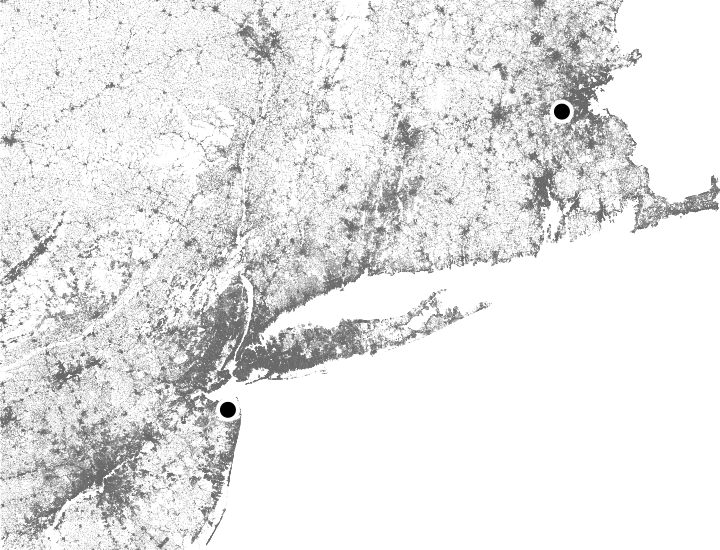
\includegraphics[width=5cm]{figs/incbi-road-ne/singleshot/example-intro.png}};
      \coordinate (s) at (1.75,0.9);
      \coordinate (t) at (3.93,2.8);
      \node (slab) at (2.5,0.6) {$s$};
      \node (tlab) at (4.0,1.5) {$t$};
      \draw[->,thick] (slab) -- (s);
      \draw[->,thick] (tlab) -- (t);
   \end{tikzpicture}%
   \caption{A graph of the Northeast USA from the 9th DIMACS
      Implementation Challenge
      comprises 1,524,453 vertices and 3,868,020 directed edges.
      A shortest path problem from a start $s$ in New Jersey
      to a destination $t$ outisde Boston
      will be used as an example.}%
   \label{fig:ibid:example-intro}%
\end{marginfigure}

\paragraph{Problem Settings.}
The single-pair problem has been extensively studied.
There are techniques that are particular to memory-constrained
settings \citep{kaindl1997biheurreconsidered}
or to settings where pre-computation is available
\citep{goldberg2007pointtopoint}.
While we do not focus on such settings,
the algorithms we propose may be complementary to these techniques.

\section{Review of Pathfinding with Distance Functions}
\label{sec:ibid:distance-functions}

This section contains a unified presentation of unidirectional,
bidirectional, and incremental search stategies
by examining the properties of the distance functions that they
maintain.
These properties and invariants can be established for arbitrary
distance function approximations.
Examination of these properties then informs the development of
algorithms which calculate them,
which we defer to Section~\ref{sef:ibid:ibid}.

While much of this section summaries prior work,
the presentation of the bidirectional termination condition
(Theorem~\ref{thm:ibid-bidir-sound}
in Section~\ref{sec:ibid:bidirectional})
in particular
is formulated to enable the novel theorems
presented in Section~\ref{sef:ibid:ibid}.

\subsection{Shortest Paths via the Start Distance Function}

\begin{marginfigure}%
   \centering%
   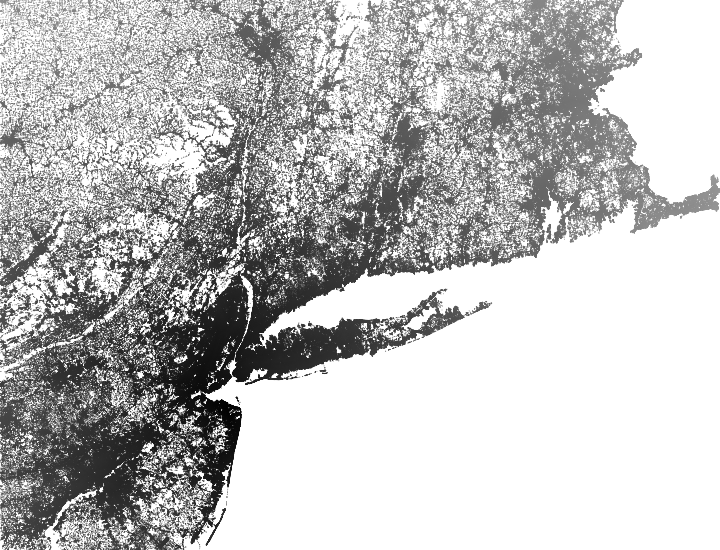
\includegraphics[width=5cm]{figs/incbi-road-ne/singleshot/example-dijkstraall.png}%
   \caption{The distance function from the start vertex.}%
   \label{fig:ibid:example-distance-all}%
\end{marginfigure}

The pioneering pathfinding algorithms of the late 1950s address
a generalization of the SPSP problem called
the \emph{single-source} problem,
where shortest paths are calculated from the start vertex $s$
to all vertices on the graph.
They proceed by calculating the \emph{start distance function}
$d^* : V \rightarrow \mathbb{R}$,
which gives the length of the shortest path from $s$
to each vertex $v$.
In other words:
\marginnote{Once the distance function $d^*$ is computed,
a shortest path to any destination $t$ can be generated trivially
by walking backwards to $s$ guided by $d^*$.}
\begin{equation}
   d^*(v) = \min_{p \in P_{sv}} \mbox{len}(p,w),
   \label{eqn:ibid-distance-function-global}
\end{equation}
where $P_{sv}$ is the set of all paths from $s$ to $v$,
and $\mbox{len}$ is given by (\ref{eqn:lazysp:len-definition})
as the sum of the path's consitutent weights
with respect to the edge weight function $w$.
Where no paths to $v$ exist,
we take $d^*(v) = \infty$.
Note that $d^*$ is only well-defined on graphs with no negative-length
cycles reachable from $s$.

Importantly, $d^*$ can also be characterized locally by
\begin{equation}
   d^*(v) = 
   \left\{ \begin{array}{cl}
      0 & \mbox{if } v = s \\
      \displaystyle\min_{u \in \mbox{\scriptsize Pred}(v)} d^*(u) + w(e_{uv}) & \mbox{otherwise,} \\
   \end{array} \right.
   \label{eqn:distance-function-char}
\end{equation}
where $\mbox{Pred}(v)$ yeilds the predecessor vertices of $v$,
and a vertex $v \neq s$ with no predecessors takes $d^*(v) = \infty$.
\marginnote{Note that
while the distance function $d^*$ necessarily satisfies
the equations (\ref{eqn:distance-function-char}),
they are not generally a sufficint condition;
if a reachable cycle of zero length exists,
(\ref{eqn:distance-function-char}) will not have a unique solution.}
The distance function is akin to the \emph{value function}
in more general decision problems addressed by dynamic programming.
The equations (\ref{eqn:distance-function-char})
are the \emph{Bellman equations} \citep{bellman1958routing},
which rely on the principle of optimality.
This characterization also follows implicitly from early results for
the all-pairs problem
\citep{shimbel1955communicationnets, beckmann1955transportation}.
Note that while (\ref{eqn:distance-function-char})
is a necessary condition of $d^*$,
it is not sufficient in general.
In particular,
if $w$ has cycles of length zero,
then even though $d^*$ is well-defined,
(\ref{eqn:distance-function-char}) admits an infinite number
of incorrect solutions for $d$.

\paragraph{Reconstructing a Shortest Path from the Distance Function.}
Calculating the start distance function is only useful for solving
the SPSP problem if it can be used to efficiently determine
a shortest path.
We can show that such a path can be reconstructed by starting at
the destination $t$ and progressively prepending the predecessor
edge $e_{uv}$ (and vertex $u$)
which locally minimizes $d^*(u) + w(e_{uv})$.
Any path constructed in this way is guaranteed to be a shortest path,
and this process is gauranteed to terminate if the graph
contains no zero-length cycles.

\subsection{Approximating $d^*$ via Tensioned Estimates}
\label{subsec:ibid-tension}

How can we compute $d^*$ efficently over the graph?
Consider an approximation function $d$
which satisfies the following four properties:%
\begin{subequations}%
   \begin{eqnarray}
      & d^*(v) \leq d(v) & \forall v
         \label{eqn:ibid-relaxation-props-nounder} \\
      & d(v) = 0 & v = s
         \label{eqn:ibid-relaxation-props-ds0} \\
      & \displaystyle\min_{u \in \mbox{\scriptsize Pred}(v)}
         d(u) + w(e_{uv}) \leq d(v)
         & v \neq s
         \label{eqn:ibid-relaxation-props-nottoogood} \\
      & d(u) + w(e_{uv}) \geq d(v) & \forall e_{uv}
         \label{eqn:ibid-relaxation-props-tens}
   \end{eqnarray}%
   \label{eqn:ibid-relaxation-props}%
\end{subequations}%
Conditions (\ref{eqn:ibid-relaxation-props-ds0} --
\ref{eqn:ibid-relaxation-props-tens})
follow directly from the local characterization
(\ref{eqn:distance-function-char});
in particular,
the case where $v \neq s$ has been split into the two
equivalent inequalities (\ref{eqn:ibid-relaxation-props-nottoogood})
and (\ref{eqn:ibid-relaxation-props-tens}).
In contrast,
for now we take the global inequality
(\ref{eqn:ibid-relaxation-props-nounder}) on faith;
we will later revisit the implications of relying on this assumption.

We can show that any estimate $d$ satisfying these properties
is the unique distance function $d^*$
via Theorem~\ref{thm:ibid-relaxation-notension}.

\begin{theorem}
\marginnote{Proofs for all theorems in this chapter are located in
Appendix~\ref{chap:appendix-ibid-proofs}.}
If $d: V \rightarrow \mathbb{R}$
satisfies (\ref{eqn:ibid-relaxation-props}),
then $d = d^*$.
\label{thm:ibid-relaxation-notension}
\end{theorem}

The principal method for arriving at an approximation
which satisfies (\ref{eqn:ibid-relaxation-props})
is via \emph{tensioned estimates}.
Consider an arbitrary approximation $d$ which satisfies only
(\ref{eqn:ibid-relaxation-props-nounder} --
\ref{eqn:ibid-relaxation-props-nottoogood}),
and consider the following edge labeling:
\begin{equation}
   \mbox{edge } e_{uv} \mbox{ is \emph{tensioned}}
   \;\;\mbox{iff}\;\;
   d(u) + w(e_{uv}) < d(v).
   \label{eqn:ibid-relaxation-tensioned}
\end{equation}
Tensioned edges are therefore those that violate
(\ref{eqn:ibid-relaxation-props-tens}).
A restatement of Theorem~\ref{thm:ibid-relaxation-notension}
is that an approximation $d$
satisfying (\ref{eqn:ibid-relaxation-props-nounder} --
\ref{eqn:ibid-relaxation-props-nottoogood})
with no tensioned edges is everywhere correct.

\paragraph{Edge Relaxation.}
How can we arrive at an approximation
satisfying Theorem~\ref{thm:ibid-relaxation-notension}?
The principal technique treats the properties
(\ref{eqn:ibid-relaxation-props-nounder} --
\ref{eqn:ibid-relaxation-props-nottoogood}) as invariants.
An initial approximation $d$ is chosen for which the invariants
trivially hold,
such as $d(v) = \infty \;\forall v \neq s$,
which will generally have many edges in tension.
The tensioned approximation $d$ is then iteratively improved
via \emph{edge relaxation}
as described by Ford \citep{ford1955networkflowtheory},
wherein a tensioned edge $e_{uv}$ is selected and relaxed
by setting $d(v) \leftarrow d(u) + w(e_{uv})$.
It can be shown that applying this process arbitrarily
maintains invariants
(\ref{eqn:ibid-relaxation-props-nounder} --
\ref{eqn:ibid-relaxation-props-nottoogood}).

It can be further shown that for a finite graph,
the number of edge relaxations needed is also finite.
The well-known Bellman-Ford method
\citep{shimbel1955communicationnets, bellman1958routing,
moore1959spmaze}
cycles through all edges repeatedly,
relaxing all tensioned edges found
(at most $|V|-1$ repetitions are sufficient for convergence).
Note that this does not place any requirements on $w$
(other than that $d^*$ must exist, so there must not be
any negative-length cycles reachable from $s$).

\begin{marginfigure}
   \centering
   \begin{tikzpicture}
      \tikzset{>=latex} % arrow heads

      \begin{scope}[shift={(0,0)}]
         \node[fill=black,circle,inner sep=1.2pt] (a) at (0,0) {};
         \node[fill=black,circle,inner sep=1.2pt] (b) at (1.5,0) {};
         \node[fill=black,circle,inner sep=1.2pt] (c) at (3.0,0) {};
         \draw[->,densely dashed] (a) -- (b) node[midway,fill=white,circle,inner sep=1pt] {1};
         \draw[->,densely dashed] (b) -- (c) node[midway,fill=white,circle,inner sep=1pt] {1};
         
         \node[above=-0.00cm of a] {$a$};
         \node[above=-0.00cm of b] {$b$};
         \node[above=-0.00cm of c] {$c$};

         \node[below=0.05cm of a] {$d=0$};
         \node[below=0.05cm of b] {$d=2$};
         \node[below=0.05cm of c] {$d=4$};
      \end{scope}

      \begin{scope}[shift={(0,-1)}]
         \node[fill=black,circle,inner sep=1.2pt] (a) at (0,0) {};
         \node[fill=black,circle,inner sep=1.2pt] (b) at (1.5,0) {};
         \node[fill=black,circle,inner sep=1.2pt] (c) at (3.0,0) {};
         \draw[->,densely dashed] (a) -- (b) node[midway,fill=white,circle,inner sep=1pt] {1};
         \draw[line width=0.10cm,black!10] (b) -- (c) node[midway,fill=white,circle,inner sep=1pt] {1};
         \draw[->] (b) -- (c) node[midway,fill=white,circle,inner sep=1pt] {1};

         \node[below=0.05cm of a] {$d=0$};
         \node[below=0.05cm of b] {$d=2$};
         \node[below=0.05cm of c] {$d=3$};
      \end{scope}

      \begin{scope}[shift={(0,-2)}]
         \node[fill=black,circle,inner sep=1.2pt] (a) at (0,0) {};
         \node[fill=black,circle,inner sep=1.2pt] (b) at (1.5,0) {};
         \node[fill=black,circle,inner sep=1.2pt] (c) at (3.0,0) {};
         \draw[line width=0.10cm,black!10] (a) -- (b) node[midway,fill=white,circle,inner sep=1pt] {1};
         \draw[->] (a) -- (b) node[midway,fill=white,circle,inner sep=1pt] {1};
         \draw[->,densely dashed] (b) -- (c) node[midway,fill=white,circle,inner sep=1pt] {1};
         
         \node[below=0.05cm of a] {$d=0$};
         \node[below=0.05cm of b] {$d=1$};
         \node[below=0.05cm of c] {$d=3$};
      \end{scope}

      \begin{scope}[shift={(0,-3)}]
         \node[fill=black,circle,inner sep=1.2pt] (a) at (0,0) {};
         \node[fill=black,circle,inner sep=1.2pt] (b) at (1.5,0) {};
         \node[fill=black,circle,inner sep=1.2pt] (c) at (3.0,0) {};
         \draw[->] (a) -- (b) node[midway,fill=white,circle,inner sep=1pt] {1};
         \draw[line width=0.10cm,black!10] (b) -- (c) node[midway,fill=white,circle,inner sep=1pt] {1};
         \draw[->] (b) -- (c) node[midway,fill=white,circle,inner sep=1pt] {1};
         
         \node[below=0.05cm of a] {$d=0$};
         \node[below=0.05cm of b] {$d=1$};
         \node[below=0.05cm of c] {$d=2$};
      \end{scope}
      
   \end{tikzpicture}
   \caption{Ordering problems.
      Consider the vertices $a \rightarrow b \rightarrow c$,
      with edges $e_{ab}$ and $e_{bc}$ both in tension;
      if $e_{bc}$ is relaxed before $e_{ab}$,
      then $e_{bc}$ will need to be relaxed a second time.}
   \label{fig:ibid:bellman-ford-repetitions}
\end{marginfigure}

\paragraph{Approximation Soundness.}
The need for multiple cycles of Bellman-Ford stems from the fact
that each edge may need to be relaxed several times.
This occurrs because relaxing an edge changes the
$d$-value of the destination vertex,
which may newly tension downstream edges
(see Figure~\ref{fig:ibid:bellman-ford-repetitions}).

We can exploit our intution to order relaxations from start to destination
in the special case where $w \geq 0$
(note that this requirement is stronger than requiring no reachable
negative-length cycles).
We can then show that our approximation $d$
is \emph{sound} for a subset of vertices
as described by Theorem~\ref{thm:ibid-relaxation-sound}.

\begin{marginfigure}
   \centering
   \includegraphics{build/ibid-dijkstra-trust}
   \caption{Tensioned edge trust region
      for $w \geq 0$.
      Contours are of the current estimate $d$.
      Currently tensioned edges are bold and dotted.}
\end{marginfigure}

\begin{theorem}
Consider $d: V \rightarrow \mathbb{R}$
satisfying (\ref{eqn:ibid-relaxation-props-nounder} --
\ref{eqn:ibid-relaxation-props-ds0}),
and let $D$ be the smallest value $d(u)$
among all tensioned edges $e_{uv}$
(or $\infty$ if no such edges exist).
If $w \geq 0$,
any vertex $x$ with $d(x) \leq D$
has $d(x) = d^*(x)$.
\label{thm:ibid-relaxation-sound}
\end{theorem}
As a result,
a given value $D$ creates a region of vertices
with values $d(x) \leq D$ that are known to be
accurate.
This confers two distinct advantages when designing an algorithm:
an efficient relaxation ordering,
and an early termination condition for single-pair problems.

\paragraph{Efficient Relaxation Ordering.}
Therefore,
all tensioned edges $e_{uv}$ with $d(u) = D$
(of which there must be at least one if any edges are tensioned)
can be relaxed immediately,
and will never be retensioned.
This is exactly the order imposed by the OPEN list in Dijkstra's
algorithm \citep{dijkstra1959anote}.

\begin{marginfigure}%
   \centering%
   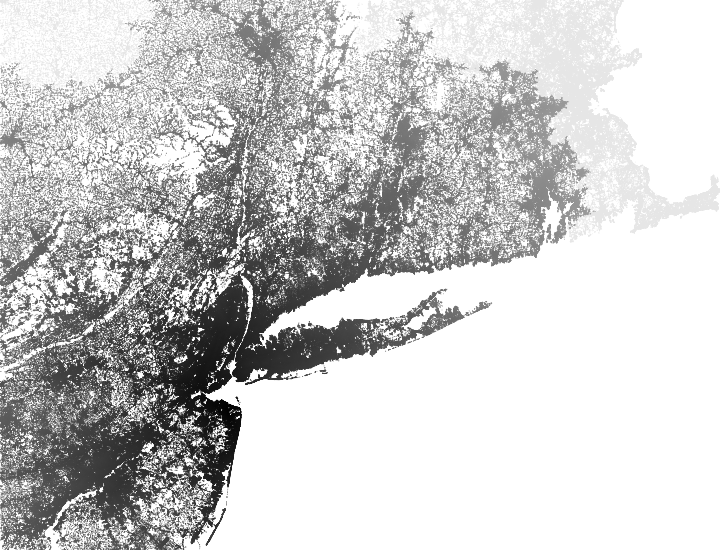
\includegraphics[width=5cm]{figs/incbi-road-ne/singleshot/example-dijkstra.png}%
   \caption{Dijkstra's algorithm computes the start distance function
      $d^*$ to solve the example shortest path problem.
      Darker vertices have smaller $d$-values.
      The algorithm stops upon reaching the destination vertex $t$
      after expanding 1,290,820 vertices.}%
   \label{fig:ibid:example-distance}%
\end{marginfigure}

\paragraph{Early Termination.}
The soundness result shows that once the destination
vertex $t$ satisfies $d(t) \leq D$,
it has the correct start distance.
Since we are only interested in reconstructing a shortest path to $t$,
we are interested in terminating computation of the distance
function as early as possible.

However,
while Theorem~\ref{thm:ibid-relaxation-sound} demonstrates
that $d(t) = d^*(t)$,
it is not by itself insufficient
to demonstrate that such a shortest path to $t$ can be reconstructed.
An illustration of such a problem case is given in
Figure~\ref{fig:ibid:relaxation-completeness-issue}.
This requres the addition of
Theorem~\ref{thm:ibid-relaxation-reconstruct} below.
Notably,
the proof for Theorem~\ref{thm:ibid-relaxation-reconstruct}
relies on (\ref{eqn:ibid-relaxation-props-nottoogood}).

\begin{marginfigure}
   \centering
   \begin{tikzpicture}
      \tikzset{>=latex} % arrow heads
      \node[fill=black,circle,inner sep=1.2pt] (s) at (0,0) {};
      \node[fill=black,circle,inner sep=1.2pt] (a) at (1.5,0) {};
      \node[fill=black,circle,inner sep=1.2pt] (b) at (1.5,1.2) {};
      \node[fill=black,circle,inner sep=1.2pt] (x) at (3.0,0) {};
      \draw[->,densely dashed] (s) -- (a) node[midway,fill=white,circle,inner sep=1pt] {0};
      \draw[->] (a) -- (x) node[midway,fill=white,circle,inner sep=1pt] {0};
      \draw[->] (s) -- (b) node[midway,fill=white,circle,inner sep=1pt] {1};
      \draw[->] (b) -- (x) node[midway,fill=white,circle,inner sep=1pt] {1};

      \node[above=0.05cm of s] {$s$};
      \node[above=0.05cm of a] {$a$};
      \node[below=0.05cm of b] {$b$};
      \node[above=0.05cm of x] {$x$};

      \node[below=0.05cm of s] {$d=0$};
      \node[below=0.05cm of a] {$d=3$};
      \node[above=0.35cm of b] {$d=1$};
      \node[below=0.05cm of x] {$d=0$};

      \node[below=0.35cm of s] {$d^*=0$};
      \node[below=0.35cm of a] {$d^*=0$};
      \node[above=0.05cm of b] {$d^*=1$};
      \node[below=0.35cm of x] {$d^*=0$};
   \end{tikzpicture}
   \caption{Problem case for pathfinding with distance functions
      in cases where invariant (\ref{eqn:ibid-relaxation-props-nottoogood})
      does not hold.
      Here, $d$ satisfied a and c, with edge $e_{sa}$ tensioned,
      and $d' = 0$.
      While the approximation $d$ is \emph{sound} at $x$
      via Theorem~\ref{thm:ibid-relaxation-sound}
      (i.e. $d(x)$ is correct),
      the path reconstructed from $t$ is not a shortest path.}
   \label{fig:ibid:relaxation-completeness-issue}
\end{marginfigure}

\begin{theorem}
Consider $d: V \rightarrow \mathbb{R}$
satisfying (\ref{eqn:ibid-relaxation-props-nounder} --
\ref{eqn:ibid-relaxation-props-nottoogood}),
and let $D$ be the smallest value $d(u)$
among all tensioned edges $e_{uv}$
(or $\infty$ if no such edges exist).
If $w \geq 0$,
for any vertex $x$ with $d(x) \leq D$,
a path reconstructed backwards from $x$ by iteratively selecting a
predecessor minimizing $d(u) + w(e_{uv})$ until $s$ is reached
is a shortest path from $s$ to $x$ of length $d^*(x)$.
\label{thm:ibid-relaxation-reconstruct}
\end{theorem}

Armed with Theorems~\ref{thm:ibid-relaxation-sound}
and~\ref{thm:ibid-relaxation-reconstruct},
we can terminate edge relaxation early
and reconstruct a shortest path from $s$ to $t$.
This algorithm is listed as ``Dijk''
(Dijkstra's algorithm)
in the results of Figure~\ref{fig:ibid:road-ne-stats}.

\subsection{Bidirectional Search}
\label{sec:ibid:bidirectional}

A prominent technique for minimizing pathfinding computation for
single-pair problems
is bidirectional search
(also called ``doubletree'' search \citep{doran1966doubletree}).
In a bidirectional algorithm,
the distance $d_t$ to the destination is calculated in a growing region
around the destination vertex $t$
concurrently with the conventional start distance $d_s$ around $s$
(Figure~\ref{fig:ibid:example-bidirectional}).
The destination distance function $d_t$,
yielding the distance of a shortest path from each vertex $u$ to $t$,
obeys a complementary definition and local characterization as $d_s$,
with vertex predecessors replaced with successors.
Approaches such as edge relaxation (Section~\ref{subsec:ibid-tension})
can therefore be used to calculate $d_t$ using a region around $t$
within which shortests paths can be reconstructed.

Loosely speaking,
the search can terminate with a shortest path
once the two regions intersect.
Each search need only descend to a depth a factor of two
shallower than a unidirectional search.
Therefore, problems where the graph density grows quickly with
the search depth are particularly well-suited to bidirectional
algorithms.
For example,
for a roadmap graph embedded in an ambient Euclidean space,
the number of expanded vertices in a ball is polynomial in the depth
and exponential in the dimensionality of the space.
It has also been empirically established that bidirectional approaches
are beneficial for instances in which many vertices around
both the start and destination vertices are costly
(e.g. due to obstacles).
This may be because the number of vertices that need to be expanded
in these regions do not grow quickly with the search depth.

\begin{marginfigure}%
   \centering%
   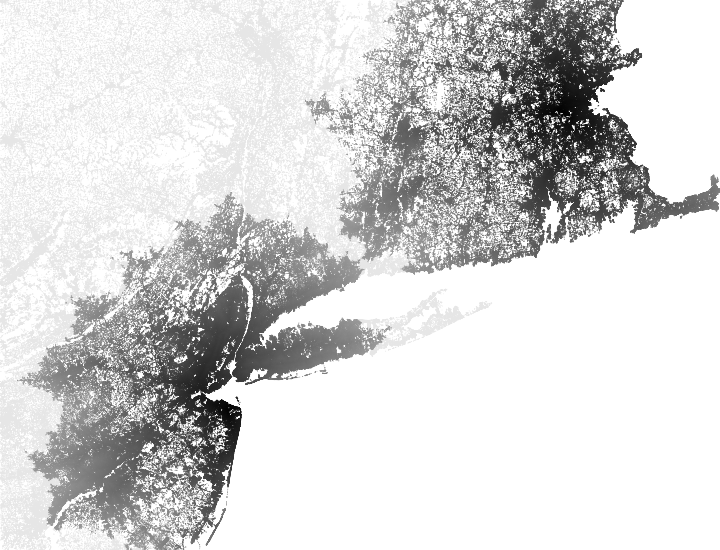
\includegraphics[width=5cm]{figs/incbi-road-ne/singleshot/example-bidijkstra.png}%
   \caption{The bidirectional Dijkatra's algorithm
      computes $d_s$ around the start vertex
      and $d_t$ around the destination vertex.
      Darker vertices have smaller $d$-values in their respective
      regions.
      The algorithm terminates after expanding a total of
      1,178,200 vertices using distance to balance expansions.}%
   \label{fig:ibid:example-bidirectional}%
\end{marginfigure}

The first bidirectional algorithm
was proposed by Dantzig \citep{dantzig1963linearprogramming},
and the first precisely described algorithm was presented by
Nicholson \citep{nicholson1966shortest},
%Implementation of a sound and efficient algorithm
%turns on two important questions:
%(a) when and how to terminate with a shortest path,
%and (b) how to balance expansions from the two directions of the
%search.
and the similar Bi-Directional Shortest Path Algorithm (BSPA)
was analyzed by Pohl \citep{pohl1971bidirectional}.
Implementation of a sound and efficient algorithm
turns on when and how to terminate with a shortest path.

\paragraph{A Correct Termination Condition.}
%\label{sec:ibid:bidirectional-termination}
What happens upon an encounter between the forward and reverse searches?
Consider running each search until the first vertex is found
that satisfies Theorem~\ref{thm:ibid-relaxation-sound} in both
directions
(that is, the first vertex $x$ for which
$d_s(x) \leq D_s$ and $d_t(x) \leq D_t$).
While Theorem~\ref{thm:ibid-relaxation-sound} correctly demonstrates
that the values $d_s(x)$ and $d_t(x)$ are correct
(and Theorem~\ref{thm:ibid-relaxation-reconstruct} similarly
demonstrates that a shortest path can be reconstructed from $s$ to $x$
and also from $x$ to $t$),
this is not sufficient to demonstrate that the shortest path
actually passes through $x$.
See Figure~\ref{fig:ibid:bidirectional-termination-issue} for a
counter-example that illustrates this point.

\begin{marginfigure}
   \centering
   \begin{tikzpicture}
      \tikzset{>=latex} % arrow heads
      \node[fill=black,circle,inner sep=1.2pt] (s) at (0,0) {};
      \node[fill=black,circle,inner sep=1.2pt] (a) at (1.5,0) {};
      \node[fill=black,circle,inner sep=1.2pt] (b) at (3.0,0) {};
      \node[fill=black,circle,inner sep=1.2pt] (t) at (4.5,0) {};
      \node[fill=black,circle,inner sep=1.2pt] (c) at (2.25,0.8) {};
      \draw[->] (s) -- (a) node[midway,fill=white,circle,inner sep=1pt] {3};
      \draw[->] (a) -- (b) node[midway,fill=white,circle,inner sep=1pt] {3};
      \draw[->] (b) -- (t) node[midway,fill=white,circle,inner sep=1pt] {3};
      \draw[->] (a) -- (c) node[midway,fill=white,circle,inner sep=1pt] {2};
      \draw[->] (c) -- (b) node[midway,fill=white,circle,inner sep=1pt] {2};
      \node[below=0.05cm of s] {$s$};
      \node[below=0.05cm of a] {$a$};
      \node[below=0.05cm of b] {$b$};
      \node[below=0.05cm of t] {$t$};
      \node[above=0.05cm of c] {$c$};
   \end{tikzpicture}
   \caption{Simple illustration of a problem case for terminating
      a bidirectional search.
      With a balanced distance criterion,
      $c$ will be the first vertex expanded in both directions,
      but it does not lie on the shortest path.}
   \label{fig:ibid:bidirectional-termination-issue}
\end{marginfigure}

Importantly, is nececessary to consider the \emph{edges} connecting
the two distance function approximations.
A correct termination condition is surprisingly subtle,%
\marginnote{There were early incorrect attempts at a sound
termination condition
\citep{berge1965programminggamestransportation}.}
with several correct variations proposed
\citep{nicholson1966shortest, dreyfus1969appraisalsp,
pohl1969bidirectional, goldberg2005spexternalmemory}.
What is necessary is a bidirectional equivalent to the 
completeness-based termination condition
from Theorem~\ref{thm:ibid-relaxation-reconstruct}.

Suppose $d_s$ and $d_t$ are approximations to $d^*_s$ and $d_t^*$,
respectively,
with each satisfying (\ref{eqn:ibid-relaxation-props}).
Let $D_s$ be the minimum $u$-value among all tensioned edges in $d_s$
(and likewise for $d_t$).
Then we can establish the following proof of a correct termination
condition:

\marginnote{This treatment of the bidirectional termination condition
is presented differently than in most related work because it will
help us formulate an incremental version
in Section~\ref{sef:ibid:ibid}.}

\begin{theorem}
Define $E_{\ms{conn}}$ as the set of all edges $e_{uv}$ such that
$d_s(u) \leq D_s$ and $d_t(v) \leq D_t$,
and define $\ell_e$ s.t. $\ell_e(e_{uv}) = d_s(u) + w(e_{uv}) + d_t(v)$.
If $w \geq 0$,
$s \neq t$,
$E_{\ms{conn}}$ is non-empty,
and $e^*_{uv}$ minimizes $\ell_e$
among $E_{\ms{conn}}$ with $\ell_e(e^*_{uv}) \leq D_s + D_t$,
then $\ell_e(e^*_{uv})$ is the length of the shortest path,
and $e^*_{uv}$ lies on one such path.
\label{thm:ibid-bidir-sound}
\end{theorem}

\paragraph{Designing an Efficient Bidirectional Algorithm.}
In the case where the approximations $d_s$ and $d_t$ are improved
via edge relaxation,
since $w \geq 0$,
by Theorem~\ref{thm:ibid-relaxation-sound}
once an edge $e_{uv}$ becomes included in
$E_{\ms{conn}}$,
its length value $\ell_e(e_{uv})$ will not change.
Therefore,
it is sufficient for a relaxation algorithm to consider only edges
newly added to $E_{\ms{conn}}$ at each iteration,
and keep track of the best edge $e^*_{uv}$
with its value $\ell_e(e^*_{uv})$ found so far.
Note also that Theorem~\ref{thm:ibid-relaxation-reconstruct}
allows a shortest path to be constructed from $e^*_{uv}$
buy walking backwards from $u$ to $s$,
and forwards from $v$ to $t$.

This algorithm is listed as ``BiDijk''
(bidirectional Dijkstra's algorithm)
in the results of Figure~\ref{fig:ibid:road-ne-stats}.

%\subsection{Balancing Directions}
%The general bidirectional algorithm leaves open the strategy
%used to balance the progression of the two search directions.
%Options based on alternating \citep{dantzig1963linearprogramming},
%or selecting the direction with the smaller {\sc Open} distance
%\citep{nicholson1966shortest}
%or {\sc Open} (and finite) set cardinality
%\citep{pohl1969bidirectional}
%have been proposed.
%Note that while some literature asserts that
%these can be interleaved arbitrarily,
%termination of the algorithm requires that each direction
%be expanded at least once.
%Our example problems use the balanced distance criterion.

\subsection{Incremental Search for Dynamic Problems}
\label{sec:ibid:incremental}

The shortest path on a graph is of course intimately tied to
the edge weight function $w$.
If the weight function changes from $w^{(1)}$ to $w^{(2)}$,
a shortest path $p^{(1)}$ w.r.t. $w^{(1)}$
will generally no longer be a shortest path w.r.t. $w^{(2)}$,
even if changes are small and localized.
For example,
if the weight of edge on $p^{(1)}$ increases,
or if the weight of some edge not on $p$ decreases,
then some other path $p^{(2)}$ may become shorter than $p^{(1)}$.
The \emph{dynamic shortest-path problem}
considers finding a shortest path
for each of a sequence of input edge weight functions.
Figure~\ref{fig:ibid:example-incremental}
shows an incremental algorithm finding a shortest path quickly
for a subsequent planning episode.

\begin{marginfigure}%
   \centering%
   \subfloat[Initial episode]{%
      \centering%
      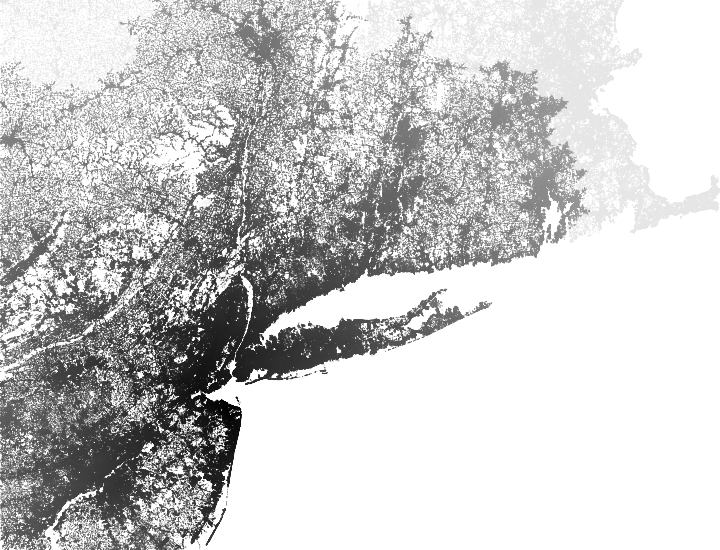
\includegraphics[width=5cm]{figs/incbi-road-ne/singleshot/example-incuni-0.png}%
   }
   
   \subfloat[Subsequent episode]{%
      \centering%
      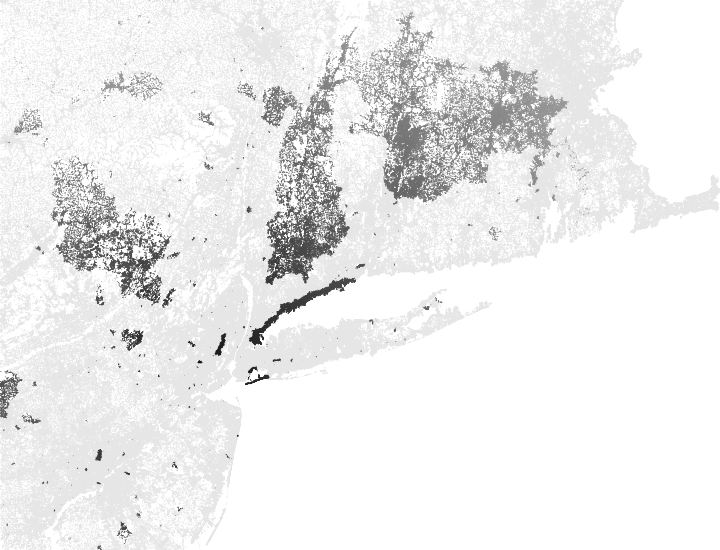
\includegraphics[width=5cm]{figs/incbi-road-ne/singleshot/example-incuni-1.png}%
   }%
   \caption{Initial episode: 1,287,897 expansions.
      Subsequent episode: 391,122 expansions.}%
   \label{fig:ibid:example-incremental}%
\end{marginfigure}

We concern ourselves with the \emph{fully dynamic} case,
in which arbitrary edge weight changes are allowed.
As mentioned in Section~\ref{subsec:ibid-probdef},
for our pathfinding problems,
we treat edges with infinite weight equivalently with non-existant
edges.
Therefore,
deleting or inserting an edge can be represented by
setting its edge weight to or from infinity, respectively.
We include here a brief review of the approach underlying common
algorithms for the dynamic pathfinding problem.

The dynamic problem has been studied in the literature.
Eary results demonstrated properties of optimal spanning trees
under certain types of update operations
\citep{spirapan1975updatingsp}.
Early algorithms considered restricted problem such as
the insert-only problem
with constant edge weights \citep{linchang1991dynamicsp},
or restricted settings such as planar graphs
\citep{klein1998planardynamicshort}.
More general algorithms followed
\citep{ramalingam1996dynamicswsffp,
   frigioni1996dynamicsinglesource,
   frigioni2000dynamicsp};
we describe and generalize the DynamicSWSF-FP algorithm
of Ramalingam and Reps below.
\marginnote{We defer for now discussing the problem of integrating
heuristic functions with incremental search;
see Section~\ref{subsec:ibid:heuristic-incremental}
for that discussion.}
A review of more general dynamic problems on graphs is available
in \citep{eppstein1999dynamic},
including for the more general all-pairs problem
\citep{demetrescu2010dynamic}.

\paragraph{Problem Definition.}
Consider a directed graph $G = (V,E)$ as described in
Section~\ref{subsec:ibid-probdef}.
Consider a sequence of pathfinding episodes
with different edge weight functions $w^{(1)}, w^{(2)}, \dots$
with $w^{(i)} : E \rightarrow \mathbb{R}$.
The dynamic single-pair shortest-path (SPSP) problem
entails finding shortest paths $p^{(1)}, p^{(2)}, \dots$
between fixed start and destination vertices $s,t \in V$
for each episode.

\paragraph{Approches to the Dynamic Problem.}
The simplest class of solutions to the dynamic SPSP problem
entails running a conventional SPSP algorithm to compute a solution
path for episode in turn.
Consider, for example, applying the edge relaxation approach
from Section~\ref{subsec:ibid-tension}
to compute the start distance function $d_s^{(i)}$ from scratch
for each episode's edge weight function $w^{(i)}$.

Investigating this approach more closely reveals an opportunity for
a more efficient algorithm.
If the changes in the weight function between each episode affect
only a subset of the edges,
then it is often the case that the value of the distance function
computed does not change for a large fraction of the vertices in the
graph.
In the face of a change in weight function
$w^{(i)} \rightarrow w^{(i+1)}$,
it is the objective of an \emph{incremental} approach
to adapt a previously computed estimate $d_s^{(i)}$
to a new one $d_s^{(i+1)}$ with a minimal amount of additional
computation.

\paragraph{Inapplicability of the Tensioned Estimates Approach.}
The tensioned estimates approach of Section~\ref{subsec:ibid-tension}
made use of two clever devices to allow its approximation $d$ to be
iteratively improved to the true distance function $d^*$.
First, it relied on a global invariant
(\ref{eqn:ibid-relaxation-props-nounder})
to ensure that the approximation was never under-consistent.
Second, it relied on a decomposition of the local characterization
(\ref{eqn:distance-function-char})
into two inequalities
(\ref{eqn:ibid-relaxation-props-nottoogood})
and (\ref{eqn:ibid-relaxation-props-tens}),
the former treated as a second invariant,
and the latter represented not as a constraint but as a labeling
of tensioned edges to be iteratively relaxed.

Unfortunately,
the incremental setting precludes this approach.
Consider a new episode in which the estimate $d^{(i+1)}$
is initialized with the preceeding estimate $d^{(i)}$.
Since the weight function $w^{(i+1)}$ has changed,
there is no guarantee that either of the invariants
(\ref{eqn:ibid-relaxation-props-nounder})
or (\ref{eqn:ibid-relaxation-props-nottoogood}) still hold.
In particular,
if edge weights increase,
it is common for one or both invariants to be violated,
and we can no longer rely on Theorems~\ref{thm:ibid-relaxation-sound}
or~\ref{thm:ibid-relaxation-reconstruct} to generate sound
shortest paths.

\paragraph{A New Approach.}
The key idea underlying the incremental approach,
and the DynamicSWSF-FP \citep{ramalingam1996dynamicswsffp} algorithm,
is to restate the local characterization (\ref{eqn:distance-function-char})
in a different way.
In particular:
\begin{subequations}%
   \begin{eqnarray}
      & r(v) = 
         \left\{ \begin{array}{cl}
            0 & \mbox{if } v = s \\
            \displaystyle\min_{u \in \mbox{\scriptsize Pred}(v)} d(u) + w(e_{uv}) & \mbox{otherwise} \\
         \end{array} \right.
         & \label{eqn:ibid-inc-props-rvalue} \\
      & d(v) = r(v)
         & \label{eqn:ibid-inc-props-consistent}
   \end{eqnarray}%
   \label{eqn:ibid-inc-props}%
\end{subequations}%
(Here, $r(v)$ represents the ``right-hand side'' of
the local characterization).
It is easy to see how (\ref{eqn:ibid-inc-props}) taken together
directly implies (\ref{eqn:distance-function-char}).
The motivation behind this decomposition is that the former
(\ref{eqn:ibid-inc-props-rvalue}) can be held as an invariant,
while the latter (\ref{eqn:ibid-inc-props-consistent})
can be established iteratively.
Prior work adopts the following labeling for each vertex $v$:
\marginnote{This meaning of consistency for vertices in incremental
search is distinct from consistency of heuristic or potential functions.}
if $d(v) = r(v)$, the vertex is \emph{consistent},
whereas inconsistent vertices are either
\emph{under-consistent} if $d(v) < r(v)$
or \emph{over-consistent} if $d(v) > r(v)$.

Importantly,
the inapplicability of the global invariant
(\ref{eqn:ibid-relaxation-props-nounder}) between episodes
has implications on the class of weight functions that can be solved
by the incremental approach.
\marginnote{Indeed,
later in Theorem~\ref{thm:ibid-dynamicswsffp-sound} we will
restrict $w$ further so that $w>0$
to garner the benefits of approximation soundness and early
termination.
However, we conjecture that the incremental algorithm is
correct even without $w>0$
(as long as no non-positive cycles exist)
as long as the algorithm is not terminated early.}
In particular,
when applied to weight functions with cycles of zero length
(for which $d^*$ is well-defined),
there is no guarantee that a distance function $d$
which satisfies (\ref{eqn:ibid-inc-props-consistent})
matches $d^*$.
We therefore restrict the class of weight functions considered
to those with only positive length cycles.

\paragraph{Approximation Soundness.}
In Section~\ref{subsec:ibid-tension},
we showed that in cases with $w \geq 0$,
the minimal value $k$ defines a trust region that can be used both
to order edge relaxations as well as inform a termination condition
after which a correct path can be reconstructed.
We can develop a similar argument about the soundness of an
approximation in the dynamic case.
In particular,
given an arbitrary estimate $d$
(and the corresponding function $r$ as defined by
(\ref{eqn:ibid-inc-props-rvalue}),
this argument makes use of a third function $k$ defined as:
\begin{equation}
   k(v) = \min\left[ d(v), r(v) \right].
   \label{eqn:ibid:incremental-key}
\end{equation}
%If we define $V_{\ms{incons}}$ as the set of inconsistent vertices
%(that is, with $d(v) \neq r(v)$,
%then we define the value $k_{\ms{min}}$ as:
%\begin{equation}
%   k_{\ms{min}} = \displaystyle\min_{v \in V_{\ms{incons}}} \left[ k(v) \right]
%\end{equation}
We can then establish the following central soundness result
for incremental search:

\begin{theorem}
Consider $d: V \rightarrow \mathbb{R}$,
with $r$ satisfying (\ref{eqn:ibid-inc-props-rvalue}),
and let $K$ be the smallest value $k(v)$
among all inconsistent vertices
(or $\infty$ if no such vertices exist).
If $w > 0$,
any consistent vertex $x$ with $d(x) \leq K$
has $d(x) = d^*(x)$.
Further,
walking backwards from $x$ choosing predecessors that minimize
$d(u) + w(e_{uv})$ terminates at $s$ with a shortest path
of length $d^*(x)$.
\label{thm:ibid-dynamicswsffp-sound}
\end{theorem}

This theorem enables the same two efficiency advantages as in
the relaxation approach, in the case where $w > 0$.
It provides that a vertex rendered consistent during an iteration
(by setting $d(x) \leftarrow r(x)$) with $d(x) \leq K$
has the correct value and will never be revisited.
It also enables an algorithm to terminate early
once the destination vertex $t$ becomes consistent,
as exploited by the Lifelong Planning A* algorithm
\citep{koenig2004lpastar}.

\subsection{Algorithm Design}

In the same way that the edge relaxation decomposition
(\ref{eqn:ibid-relaxation-props}) allowed way to progressively
update an estimate $d$ via a priority queue,
the decomposition (\ref{eqn:ibid-inc-props}) affords the same
opportunity.
The DynamicSWSF-FP algorithm \citep{ramalingam1996dynamicswsffp}
maintains a queue $Q$ of inconsistent vertices,
and processes them in the order given by the priority key
(\ref{eqn:ibid:incremental-key})
used in the soundness result
in Theorem~\ref{thm:ibid-dynamicswsffp-sound}.

One key aspect of the algorithm is the way underconsistent vertices
are handled.
Upon encountering an underconsistent vertex ($d(v) < r(v)$),
the algorithm applies $d(v) \leftarrow \infty$
(if the vertex remains inconsistent, it would be rendered
consistent in a future iteration if necessary).
This ensures that each vertex is processed at most twice during
each planning episode.
This algorithm is listed as ``DynSWSF''
(Dynamic SWSF-FP)
in the results of Figure~\ref{fig:ibid:road-ne-stats}.

% I don't need this anymore, subsumed in soundness result!
%\paragraph{Approximation Completeness.}
%
%For bidirectional search,
%it's also necessary to be able to prove that you have found
%all vertices within a certain distance of the start.
%Basically, this is a completeness proof --
%if a distance exists below a certain value,
%we will have found it.
%This is completeness of the approximation,
%not of an algorithm per se.
%
%\begin{theorem}
%Any vertex $x$ with $d^*(x) < k_{\ms{min}}$
%has $d(x) = d^*(x)$.
%\label{thm:ibid-dynamicswsffp-complete}
%\end{theorem}
%
%\begin{proof}[Proof of Theorem~\ref{thm:ibid-dynamicswsffp-complete}]
%We show that $d(x)$ can be both
%no less than $d^*(x)$
%(Lemma~\ref{lemma:ibid-dynamicswsffp-complete-geq})
%and no greater than $d^*(x)$
%(Lemma~\ref{lemma:ibid-dynamicswsffp-complete-leq}).
%\end{proof}
%
%\begin{lemma}
%Any vertex $x$ with $d^*(x) < k_{\ms{min}}$
%has $d(x) \geq d^*(x)$.
%\label{lemma:ibid-dynamicswsffp-complete-geq}
%\end{lemma}
%
%\begin{proof}[Proof of Lemma~\ref{lemma:ibid-dynamicswsffp-complete-geq}]
%We show this by contradiction.
%Suppose there exists a vertex $x$ with $d^*(x) < k_{\ms{min}}$
%for which $d(x) < d^*(x)$.
%Then $d(x) < k_{\ms{min}}$,
%so $x$ must be consistent.
%By Lemma~\ref{lemma:ibid-dynamicswsffp-sound-geq},
%we must have $d(x) \geq d^*(x)$.
%This contradicts our supposition.
%\end{proof}
%
%\begin{lemma}
%Any vertex $x$ with $d^*(x) < k_{\ms{min}}$
%has $d(x) \leq d^*(x)$.
%\label{lemma:ibid-dynamicswsffp-complete-leq}
%\end{lemma}
%
%\begin{proof}[Proof of Lemma~\ref{lemma:ibid-dynamicswsffp-complete-leq}]
%This proof proceeds in a similar way to that for
%Lemma~\ref{lemma:ibid-dynamicswsffp-sound-leq}.
%Construct a true shortest path from $s$ to $x$,
%with $d^*$-values increasing monotonically from
%$d^*(s) = 0$ to $d^*(x)$.
%Consider each edge $e_{uv}$ in turn as follows.
%Assume that $u$ is consistent,
%with $d(u) \leq d^*(u)$.
%Note that this is true for the first edge with $u = s$,
%since with $0 \leq d^*(x)$,
%we have $0 < k_{\ms{min}}$,
%so that $s$ must is consistent with $r(s) = d(s) = d^*(s) = 0$.
%Since $e_{uv}$ lies on a true shortest path,
%we must have $d^*(u) + w(e_{uv}) = d^*(v)$,
%and for all edges $d(u) + w(e_{uv}) \geq r(v)$.
%Together, this implies that
%$d^*(u) - d(u) \leq d^*(v) - r(v)$.
%Our assumption that $d(u) \leq d^*(u)$
%therefore implies that $r(v) \leq d^*(v)$.
%Since $d^*(v) \leq d^*(x)$ and $d^*(x) < k_{\ms{min}}$,
%we know that $v$ is consistent,
%so we conclude that $d(v) \leq d^*(v)$,
%and we can proceed to the next edge on the path.
%We end with $v = x$,
%so that $d(x) \leq d^*(x)$.
%\end{proof}

\section{Incremental Bidirectional Search}
\label{sef:ibid:ibid}

The principal motivation behind
the Incremental Bidirectional (IBiD) search algorithm
is to leverage the early termination efficiency of a bidirectional search
with the efficiency of an incremental search for dynamic
single-pair shortest path problems.
An example of IBiD is shown in
Figure~\ref{fig:ibid:example-incremental-bidirectional}.
\begin{marginfigure}%
   \centering%
   \subfloat[Initial search]{%
      \centering%
      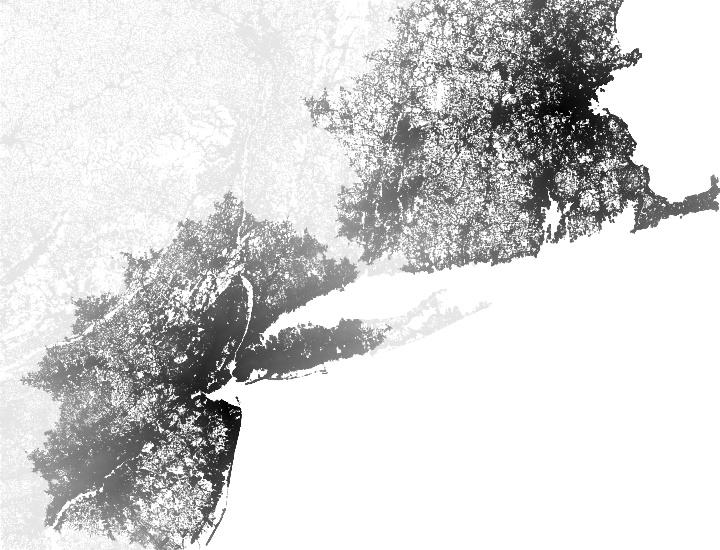
\includegraphics[width=5cm]{figs/incbi-road-ne/singleshot/example-incbi-0.png}%
   }
   
   \subfloat[Replan search]{%
      \centering%
      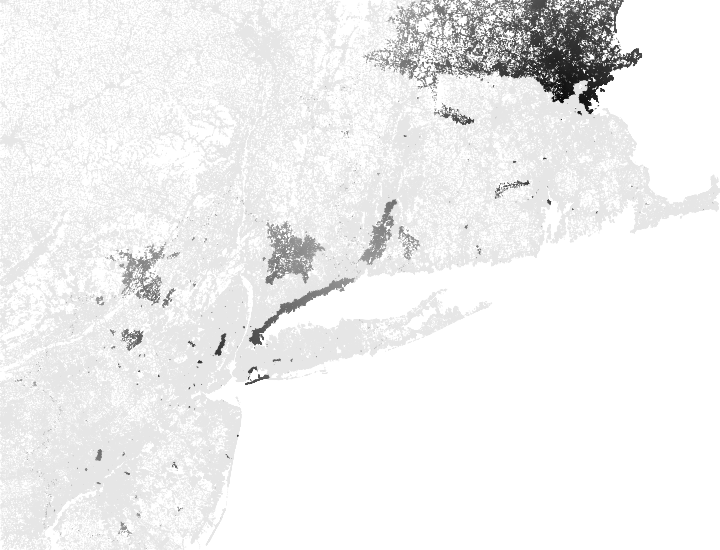
\includegraphics[width=5cm]{figs/incbi-road-ne/singleshot/example-incbi-1.png}%
   }%
   \caption{Initial search: 1,181,616 expansions.
      Replan: 262,422 expansions.}%
   \label{fig:ibid:example-incremental-bidirectional}%
\end{marginfigure}

Because it is derived from DynamicSWSF-FP,
the IBiD algorithm is applicable to graphs with $w > 0$.
(If zero weights are present,
the algorithm can be adapted by transforming $w$ to use
lexographically sorted tuples as developed
by LPA* \citep{koenig2004lpastar},
described in Section~\ref{subsec:ibid:heuristic-incremental}.)
Note also that as an extension of
Bidirectional Dijkstra's algorithm \citep{goldberg2005spexternalmemory},
the algorithm presented requires $s \neq t$.
If the start and destination vertices coincide,
an empty path can be returned in a preprocessing step.

\subsection{Bidirectional Termination with Incremental Distance Functions}

Consider a graph endowed with two distance functions,
a start distance approximation $d_s$,
and a destination distance approximation $d_t$.
Since this is an incremental setting,
we can make use of the formulation
of Theorem~\ref{thm:ibid-dynamicswsffp-sound}
from Section~\ref{sec:ibid:incremental}
to establish the correctness of these approximations
for certain vertices.

It is essential that the bidirectional termination condition from
Theorem~\ref{thm:ibid-bidir-sound} be adapted to
handle these incrementally maintained distance functions.
The central theorem that enables the IBiD algorithm is:

\begin{theorem}
Consider a graph with $w > 0$ and with $s \neq t$.
Consider a start distance approximation $d_s: V \rightarrow \mathbb{R}$,
with $r_s$ satisfying (\ref{eqn:ibid-inc-props-rvalue}),
and let $K_s$ be the smallest value $k_s(v)$
among all inconsistent vertices,
or $\infty$ if no such vertices exist;
likewise, consider the same for a destination distance approximation
$d_t$ and its accompanying $r_t$ and $K_t$.

Define $E_{\ms{conn}}$ as the set of all edges $e_{uv}$ such that
$u$ is $s$-consistent with $d_s(u) \leq K_s$
and $v$ is $t$-consistent with $d_t(v) \leq K_t$,
and define $\ell_e$ s.t. $\ell_e(e_{uv}) = d_s(u) + w(e_{uv}) + d_t(v)$.
If $E_{\ms{conn}}$ is non-empty,
and $e^*_{uv}$ minimizes $\ell_e$
among $E_{\ms{conn}}$ with $\ell_e(e^*_{uv}) \leq K_s + K_t$,
then $\ell_e(e^*_{uv})$ is the length of the shortest path,
and $e^*_{uv}$ lies on one such path.
\label{thm:ibid-sound}
\end{theorem}

Note that the first half of the conditions
from Theorem~\ref{thm:ibid-sound}
is drawn from the soundness conditions for incremental search
from Theoem~\ref{thm:ibid-dynamicswsffp-sound},
while the second half resembles the bidirectional termination
conditions from Theorem~\ref{thm:ibid-bidir-sound}.

\subsection{Algorithm Design}

{\floatevery{algorithm}{\setlength\hsize{16.85cm}}
\begin{algorithm}[t]
   \caption{As a bidirectional algorithm,
      IBiD conducts two independent DynamicSWSF-FP searches,
      one computing distance from the start vertex $s$,
      and the other computing distance to the destination vertex $t$.}
   \label{alg:ibid-two-dynamicswsffps}
   \begin{minipage}[t]{8.2cm}
      \begin{algorithmic}[1]
         \Procedure {InitializeStart} {\,\!}
            \ForAll {$v \in V$}
               \State $d_s(v) \gets \infty; \;\; r_s(v) \gets \infty$
            \EndFor
            \State $r_s(s) \gets 0$
            \State $Q_s \gets \{ s \}$
               \Comment $\mbox{ key for } v: \min\big(r_s(v),d_s(v)\big)$
            \State $\mbox{\sc ProcessStartQueue}()$
         \EndProcedure
         \Procedure {UpdateStartDistance} {$v$}
            \If {$v \neq s$}
               \State $r_s(v) \gets \displaystyle\min_{u \in \mbox{\scriptsize Pred}(v)}
                  \big( d_s(u) + w(u,v) \big)$
            \EndIf
            \State Ensure $v \in Q_s$ iff $d_s(v) \neq r_s(v)$
         \EndProcedure
         \Procedure {ProcessStartQueue} {\,\!}
            \State $u \gets Q_s.\mbox{Pop}()$
            \If {$r_s(u) < d_s(u)$}
                  \Comment over-consistent
               \State $d_s(u) \gets r_s(u)$
               \ForAll {$v \in \mbox{Succ}(u)$}
                  \State $\mbox{\sc UpdateStartDistance}(v)$
               \EndFor
            \Else
                  \Comment under-consistent
               \State $d_s(u) \gets \infty$
               \ForAll {$v \in \mbox{Succ}(u) \cup u$}
                  \State $\mbox{\sc UpdateStartDistance}(v)$
               \EndFor
            \EndIf
         \EndProcedure
         \algstore{ibid-two-dynamicswsffps}
      \end{algorithmic}
   \end{minipage}
   \quad
   \begin{minipage}[t]{8.2cm}
      \begin{algorithmic}[1]
         \algrestore{ibid-two-dynamicswsffps}
         \Procedure {InitializeDest} {\,\!}
            \ForAll {$v \in V$}
               \State $d_t(v) \gets \infty; \;\; r_t(v) \gets \infty$
            \EndFor
            \State $r_t(t) \gets 0$
            \State $Q_t \gets \{ t \}$
               \Comment $\mbox{ key for } v: \min\big(r_t(v),d_t(v)\big)$
            \State $\mbox{\sc ProcessDestQueue}()$
         \EndProcedure
         \Procedure {UpdateDestDistance} {$u$}
            \If {$u \neq t$}
               \State $r_t(u) \gets \displaystyle\min_{v \in \mbox{\scriptsize Succ}(u)}
                  \big( w(u,v) + d_t(v) \big)$
            \EndIf
            \State Ensure $u \in Q_t$ iff $d_t(u) \neq r_t(u)$
         \EndProcedure
         \Procedure {ProcessDestQueue} {\,\!}
            \State $v \gets Q_t.\mbox{Pop}()$
            \If {$r_t(v) < d_t(v)$}
                  \Comment over-consistent
               \State $d_t(v) \gets r_t(v)$
               \ForAll {$u \in \mbox{Pred}(v)$}
                  \State $\mbox{\sc UpdateDestDistance}(u)$
               \EndFor
            \Else
                  \Comment under-consistent
               \State $d_t(v) \gets \infty$
               \ForAll {$u \in \mbox{Pred}(v) \cup v$}
                  \State $\mbox{\sc UpdateDestDistance}(u)$
               \EndFor
            \EndIf
         \EndProcedure
      \end{algorithmic}
   \end{minipage}
\end{algorithm}
} % floatevery width adjustment

\paragraph{Simultaneous Incremental Searches.}
The IBiD algorithm runs two independent conventional
DynamicSWSF-FP \citep{ramalingam1996dynamicswsffp}
searches simultaneously,
one from the start vertex $s$
and one from the destination vertex $t$,
with each maintaining a separate priority queue of
inconsistent vertices $Q_s$ and $Q_t$ respectively
(Algorithm~\ref{alg:ibid-two-dynamicswsffps}).

As with a convential bidirectional search,
the two sides can be alternated arbitrarily,
except that the each queue must be processed once upon initialization
so that $d_s(s) = 0$ and $d_t(t) = 0$.

\paragraph{Remembering Connections.}
Theorem~\ref{thm:ibid-sound} has ramifications when designing
an algorithm.
In the case of bidirectional search
described in Section~\ref{sec:ibid:bidirectional},
the algorithm could take a shortcut since $D$-values always decreased,
so it was not necessary to remember older edges when better
ones were found.
In the incremental case,
where the start and destination distance functions $d_s$ and $d_t$
may both increase and decrease between episodes,
it is no longer sufficient to remember only the best connection
found so far.

Instead,
we track all potential connection edges in a connection queue $Q_c$.
Members of this queue are edges on the graph $e_{uv}$
for which vertex $u$ is $s$-consistent,
and vertex $v$ is $t$-consistent.
This queue is sorted bythe key $d_s(u) + w(u,v) + d_t(v)$.
As an optimization,
the queue does not include edges for which the key is infinite,
since that corresponds to a non-existant path.
The resulting algorithm outline is shown in Algorithm~\ref{alg:ibid}.

\begin{algorithm}[t]
   \caption{IBiD Outline}
   \label{alg:ibid}
   \begin{algorithmic}[1]
      \Procedure {Main} {\,}
         \State $\mbox{\sc InitializeStart}(); \; \mbox{\sc InitializeDest}()$
         \State $Q_c \gets \emptyset$
            \Comment $\mbox{ key for } (u,v): d_s(u) + w(u,v) + d_t(v)$
         \Loop
            \While {not $\mbox{\sc TerminationCondition}()$}
               \If {$Q_s.\mbox{TopKey} < Q_t.\mbox{TopKey}$}
                     \Comment prioritize arbitrarily
                  \State $\mbox{\sc ProcessStartQueue}(u)$
               \Else
                  \State $\mbox{\sc ProcessDestQueue}(u)$
               \EndIf
               \State Ensure $(u,v) \in Q_c$ iff
                  $u \neq Q_s$, $v \neq Q_t$, key $\neq \infty$
            \EndWhile
            \State $(u_c,v_c) \gets Q_c.\mbox{Top}$
            \State $\pi \gets
               ( \mbox{walk } d_s \mbox{ from } u_c \mbox{ to } s )
               \cup
               ( \mbox{walk } d_t \mbox{ from } v_c \mbox{ to } t )$
            \State wait for edges $(u,v) \in E_{\ms{delta}}$ with changed weights $w(u,v)$
            \State $\mbox{\sc NotifyWeightChanges}(E_{\ms{delta}})$
         \EndLoop
      \EndProcedure
      \Procedure {NotifyWeightChanges} {$E_{\ms{delta}}$}
         \ForAll {$(u,v) \in E_{\ms{delta}}$}
            \State $\mbox{\sc UpdateStargDistance}(v)$
            \State $\mbox{\sc UpdateDestDistance}(u)$
         \EndFor
         \State Ensure $(u,v) \in Q_c$ iff
            $u \neq Q_s$, $v \neq Q_t$, key $\neq \infty$
      \EndProcedure
   \end{algorithmic}
\end{algorithm}

\paragraph{Termination Condition.}
The termination condition from Theorem~\ref{thm:ibid-sound}
is captured in Algorithm~\ref{alg:ibid:ibid-termination}.
The first conditional handles cases where no finite path exists.
This algorithm is listed as ``IBiD''
in the results of Figure~\ref{fig:ibid:road-ne-stats}.

\begin{algorithm}
   \caption{IBiD Termination Condition}
   \label{alg:ibid:ibid-termination}
   \begin{algorithmic}[1]
      \Function {TerminationCondition} {\,}
         \If {$\left[Q_s.\mbox{Empty} \mbox{\bf{ and }} d_s(t)\!=\!\infty\right]$
            {\bf or} $\left[Q_t.\mbox{Empty} \mbox{\bf{ and }} d_t(s)\!=\!\infty\right]$}
            \State \Return True
               \Comment no solution path
         \EndIf
         \State $(u_c,v_c) \gets Q_c.\mbox{TopKey}$
            \Comment return False if $Q_c$ empty
         \If {$Q_s.\mbox{TopKey} + Q_t.\mbox{TopKey} < d_s(u_c) + w(u_c,v_c) + d_t(v_c)$}
            \State \Return False
         \EndIf
         \If {$Q_s.\mbox{TopKey} < d_s(u_c)$
               \mbox{\bf or} $Q_t.\mbox{TopKey} < d_t(v_c)$}
            \State \Return False
         \EndIf
         \State \Return True
      \EndFunction
   \end{algorithmic}
\end{algorithm}

\section{Heuristic Search}
\label{sec:ibid:heuristic}

When examining how to assemble a heuristic-informed algorithm
that integrates bidirectional with incremental methods,
it's instructive to examine how these efforts have been addressed
in the past.

\paragraph{Review of Heuristic Methods.}
Heuristic methods such as the Graph Traverser
\citep{doran1966graphtraverser} were originally
applied to pathfinding problems in order to find non-optimal
solutions more economically.
These unidirectional methods proceed similarly to Dijkstra's algorithm,
but instead of prioritizing {\sc Open} vertices
based on their start distance $d_s$,
they use a destination-directed heuristic function $h_t$.
Hart, Nilsson, and Raphael \citep{hart1968astar} established that
these approaches can be combined ($d_s + h_t$) to yield
an admissible algorithm (A*) for the shortest-path problem,
as long as $h_t$ meets certain conditions.
See Figure~\ref{fig:ibid:example-astar}.
We show the results of unidirectional heuristic search as ``A*''
in the results of Figure~\ref{fig:ibid:road-ne-stats}.

\begin{marginfigure}%
   \centering%
   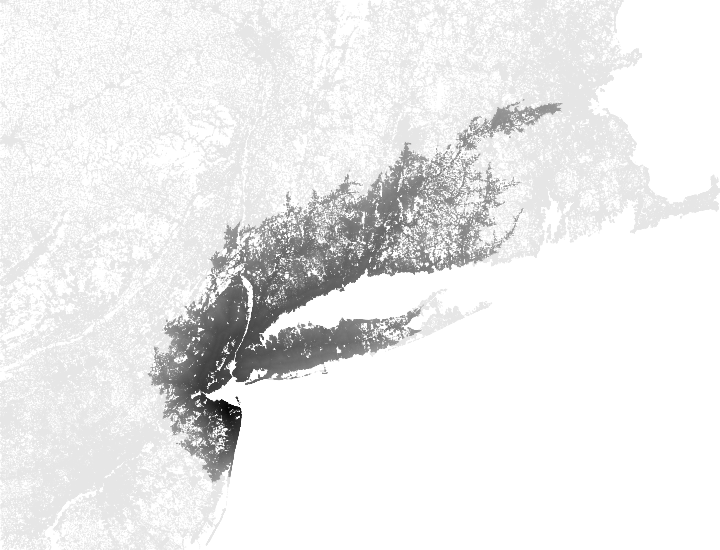
\includegraphics[width=5cm]{figs/incbi-road-ne/singleshot/example-astar.png}%
   \caption{A* search.
      532,880 expansions.}%
   \label{fig:ibid:example-astar}%
\end{marginfigure}

\subsection{Heuristic Methods in Bidirectional Search}
\label{subsec:ibid:heuristic-bidirectional}

Attempts to provide a bidirectional algorithm which incorporates
heuristic estimates generally take one of three approaches,
which we survey here.

First,
``front-to-back'' methods
such as Pohl's Bidirectional Heuristic Path Algorithm (BHPA)
\citep{pohl1971bidirectional}
conduct two conventional heuristic-informed searches
(i.e. the start search directed to the destination vertex,
and vice versa).
This approach suffers from the problem that the two sets of
\textsc{Closed} vertices must overlap substantially
before the search can be terminated,
and therefore the benefit of the bidirectional search
is not fully realized.
%\cdnote{Pohl cites Berge? Missile analogy.}

Second,
``front-to-front'' methods exploit a pairwise
heuristic function $h(u,v)$ evaluated over every pair of vertices
on each search's \textsc{Open} list,
and the vertices representing the shortest potential path are
expanded.
Early approaches with inflated heuristics
\citep{doran1966doubletree} did not yield promising results.
The later Bidirectional Heuristic Front-to-Front Algorithm
(BHFFA) \citep{champeaux1983biheuragain} does show an improved
number of vertex expansions.
\marginnote{An earlier version of BHFFA \citep{champeauxsint1977bhffa}
was shown to be incorrect due in large part to the difficulty
establishing a correct bidirectional termination condition.}
While this approach does not suffer from the region overlap problem
inherent in front-to-back methods,
it instead incurrs the very high cost of computing full pairwise
heuristics, and updating all vertices on \textsc{Open}
after each vertex expansion.

The third approach
derives from an alternative interpretation of heuristic search
algorithms first proposed by Ikeda et. al.
\citep{ikeda1994betterroutes}.
Under this interpretation,
a heuristic-informed A* search is equivalent to an uninformed
Dijkstra's search under a particular transformation
of the edge weights using the heuristic function
as a vertex potential function.
Therefore,
because front-to-back methods use different heuristics for the
forward and reverse searches,
they are effectively searching graphs with different weight functions.
The proposed solution is to arrive at a single consistent potential
function,
which allows the transformed pathfinding problem to be solved using
the uninformed bidirectional algorithm described
in Section~\ref{sec:ibid:bidirectional}.

\paragraph{Potential-Adjusted Weight Functions.}
Consider an arbitrary vertex potential function
$b : V \rightarrow \mathbb{R}$,
and consider the following transformation of a weight
function $w$ into transformed weight function $w_b$:
\begin{equation}
   w_b(e_{uv}) = w(e_{uv}) - \left[ b(u) - b(v) \right].
   \label{eqn:ibid:potential-transformation}
\end{equation}
The effect of this transformation on the lengths of paths over $G$
bears investigation.
Consider a path $p_{xy}$ from $x$ to $y$ which has length $\ell$ w.r.t. $w$.
What is its weight $\ell_b$ w.r.t. $w_b$?
A simple summation reveals that
\begin{equation}
   \ell_b(p_{xy}) = \ell(p_{xy}) - \left[ b(x) - b(y) \right].
   \label{eqn:ibid:potential-path-lengths}
\end{equation}
That is, the difference between the initial and transformed lengths
of the path from $x$ to $y$ is independent of the path itself
(its consituent vertices and edges),
and only a function of the endpoint vertices.
In particular,
this implies that a shortest path from $x$ to $y$ w.r.t. $w_b$
remains a shortest path w.r.t. $w$.
Therefore, any admissible shortest path algorithm can be used to
solve w.r.t. $w_b$.
Note that the transformation does not change the length of any
cycles in $G$.
Note also that as a consequence of
(\ref{eqn:ibid:potential-path-lengths}),
the original and transformed start distance functions are related by
\begin{equation}
   d^*_b(v) = d^*(v) - \left[ b(s) - b(v) \right].
\end{equation}

\paragraph{Benefit of Potential Adjustment.}
If the ordering of solution paths does not change under the
potential function transformation,
what benefit would be obtained by conducting the search
on the transformed weight function?
Indeed,
computing the full distance function $d_s$ over $w_b$,
e.g. by edge relaxation,
appears just as expensive.

The key insight is that under an appropriately chosen potential function,
many shortest path algorithms are able to terminate more quickly.
To see why,
consider the potential function $b$ coinciding with
the destination heuristic function $h_t$ used in A*.
By (\ref{eqn:ibid:potential-transformation}),
the weight $w_b$ of a directed edge $e_{uv}$ which makes
progress towards the destination (so that $b(v) < b(u)$)
will have its transformed weight be reduced,
whereas an edge in the incorrect direction will have its transformed
weight increase.
The transformed quantity $w_b$
from (\ref{eqn:ibid:potential-transformation})
can be considered the \emph{excess weight} of each edge,
relative to the expected weight given the progress measured by the
heuristic function
(this quantity has also been called the ``waste'' of the edge
\citep{pohl1969bidirectional}).
A pathfinding algorithm therefore searches only in the excess weight
space,
and is therefore biased to explore paths which make progress towards
the destination vertex.
In effect,
while the transformation does not affect the relative ordering of
paths,
it does shift the weight between edges on paths to accentuate poor
choices to allow for early termination.

\paragraph{Requirements on the Potential Function.}
The argument that ordering of paths (and therefore shortest path(s))
is invariant to the transformation is true for any arbitrary
potential function.
However,
in order to be useful,
we must be able to solve the transformed problem efficiently
(i.e. with early termination).
As we saw for edge relaxation in Section~\ref{subsec:ibid-tension},
our soundness result from Theorem~\ref{thm:ibid-relaxation-reconstruct}
requires that the edge weight function be nonnegative.
This induces the requirement that
the vertex potential $b$ to be \emph{consistent}
(also known as \emph{monotone} or \emph{dual feasible}), i.e.
\begin{equation}
   b(u) + w(e_{uv}) \geq b(v) \quad\forall e_{uv} \in E.
   \label{eqn:ibid:potential-consistent}
\end{equation}
If (\ref{eqn:ibid:potential-consistent}) holds,
then the efficient ordering and early termination
for edge relaxation (i.e. Dijkstra's algorithm)
can be applied to the transformed problem $w_b$,
and the returned path is also a shortest path w.r.t. $w$. 

\paragraph{Potential Functions for Bidirectional Search.}
Treating heuristic search as such a potential function transformation
allows Ikeda et. al. \citep{ikeda1994betterroutes} to apply
the same idea to bidirectional search.
In particular,
if one commits to a single potential function $b$,
then the conventional bidirectional algorithm
(Section~\ref{sec:ibid:bidirectional})
can be applied directly.
The question is,
what potential function should we use?

A bidirectional search customarily has available
two heuristic functions,
one $h_t(v)$ that approximates the length of paths
from $v$ to the destination vertex $t$,
and one $h_s(v)$ that approximates the length of paths
from the start vertex to $v$.
The most commonly used potential function
\citep{ikeda1994betterroutes, goldberg2005spexternalmemory}
is simply the average of the two:
\begin{equation}
   b(v) = \frac{h_t(v) - h_s(v)}{2}.
   \label{eqn:ibid:averaged-potential}
\end{equation}
Note that the start heuristic value is negated;
when the start heuristic is used during the reverse search,
it is applied to predecessor vertices.
It can be shown that if $h_s$ and $h_t$ are consistent
(i.e. satisfy (\ref{eqn:ibid:potential-consistent})),
$b$ is also consistent.

\begin{figure}
   \centering%
   
   \includegraphics{build/incbi-lpastar-fig1/lpastar-heurnone-original}%
   \;\;%
   \includegraphics{build/incbi-lpastar-fig1/incbi-heurnone-original}%
   
   %\vspace{0.2cm}
   %
   %\includegraphics{build/incbi-lpastar-fig1/lpastar-heurhalf-original}%
   %\;\;%
   %\includegraphics{build/incbi-lpastar-fig1/incbi-heurhalf-original}%
   
   \vspace{0.2cm}
   
   \includegraphics{build/incbi-lpastar-fig1/lpastar-heurfull-original}%
   \;\;%
   \includegraphics{build/incbi-lpastar-fig1/incbi-heurfull-original}%
   
   \caption{Illustration of behavior of bidirectional heuristic serach
      on a shortest path problem reproduced
      from \citep{koenig2004lpastar}.
      Vertices that are start-expanded are shown in blue,
      while those that are destination-expanded are shown in red.
      At left, the algorithm performs only start-side expansions,
      which approximates the behavior of a unidirectional algorithm.
      At right, the algorithm  performs distance-balanced expansions
      between the two searches.
      The top row shoes the behavior of the algorithm with no
      heuristic potential function.
      Start and destination heuristic functions are available,
      and their effect are shown at bottom.
      The unidirectional search uses the destination heuristic $h_t$
      as its potential function,
      while the bidirectional search uses the averaged potential
      function (\ref{eqn:ibid:averaged-potential}).
      }
   \label{fig:incbi-lpastar-fig1-heurchange}
\end{figure}

Figure~\ref{fig:incbi-lpastar-fig1-heurchange} shows the behavior
of the bidirectional heuristic search algorithm
on a path planning problem in an eight-connected grid world.
This example problem is reproduced from \citep{koenig2004lpastar}.
The figure shows the effect of the combination of bidirectional
and heuristic search.

Figure~\ref{fig:ibid:example-heurbidijkstra} shows the result
of conducting a bidirectional search using this averaged
potential function for the example road network problem.
This algorithm is listed as ``H-BiDijk''
(heuristic bidirectional Dijkstra's)
in the results of Figure~\ref{fig:ibid:road-ne-stats}.

\begin{marginfigure}%
   \centering%
   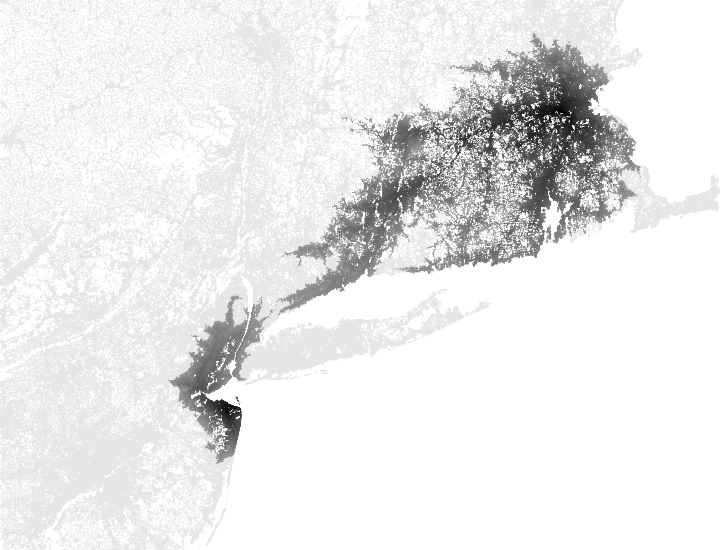
\includegraphics[width=5cm]{figs/incbi-road-ne/singleshot/example-heurbidijkstra.png}%
   \caption{Bidirectional A* search.
      515,588 expansions.}%
   \label{fig:ibid:example-heurbidijkstra}%
\end{marginfigure}

% \cdnote{To integrate: \citep{dechter1984bfsastaropt}.}

\subsection{Heuristic Methods in Incremental Search}
\label{subsec:ibid:heuristic-incremental}

Efforts to integrate heuristics into incremental search algorithms
have taken a similar potential function approach.
Koenig et. al. developed Lifelong Planning A* \citep{koenig2004lpastar},
which implicitly applies this transformation
and then applies the DynamicSWSF-FP incremental algorithm
\citep{ramalingam1996dynamicswsffp}
from Section~\ref{sec:ibid:incremental}
to solve the dynamic problem.
However,
the underlying incremental algorithm has a stricter requirements:
while Dijkstra's algorithm requires $w \geq 0$,
Theorem~\ref{thm:ibid-dynamicswsffp-sound} governing
the incremental algorithm requires $w > 0$.
As a result,
even in the case where the potential function is consistent
via (\ref{eqn:ibid:potential-consistent}),
the transformed weight function $w_b$ will not generally satisfy
$w_b > 0$.
This occurs along all edges for which the weight is identical to
the potential function difference
-- exactly the expected scenario when the potential function is
accurate.

\paragraph{Avoiding the Zero Weight with Sorted Tuples.}
LPA* solves the zero weight problem by effectively conducting
the incremental search over a different set of edge weights --
instead of the reals $w : E \rightarrow \mathbb{R}^{> 0}$,
each transformed edge weight is instead a member of a product space
\begin{equation}
   w_b \;:\; E \;\rightarrow\; \mathbb{R}^{\geq 0} \!\times\! \mathbb{R}^{> 0}.
\end{equation}
with the transformation defined as
\begin{equation}
   w_b(e_{uv}) = \big[ w(e_{uv}) - [b(u) - b(v)]; \; w(e_{uv}) \big].
   \label{eqn:ibid:incremental-potential-key}
\end{equation}
Note that the first element of the tuple concides with the
non-incremental potential function transformation from
(\ref{eqn:ibid:potential-transformation}).
Elements of the product space are sorted lexographically;
that is, their comparison only considers the first component,
with the exception that when the first component is equal,
the second component is then considered.
Summing two elements is performed component-wise.
\marginnote{Note that in order to maintaion $w_b > 0$,
the second element need only be positive,
and could even be constant (e.g. unity).
We keep the value $w(e_{uv})$ for consistency with LPA*.}
Note that since the we already assert that $w > 0$ for incremental
domains,
the second component of $w_b$ is everywhere positive,
and therefore $w_b > (0,0)$.

\paragraph{Equivalence to Lifelong Planning A*}
Our treatment of the transformed edge weight function $w_b$
and the key function $k$ differs from the original presentation
\citep{koenig2004lpastar}.
Here,
we will briefly show that they are equivalent.

Consider two algorithms conducting a search over a graph:
(a) LPA*
and (b) DynamicSWSF-FP with its incremental key
(\ref{eqn:ibid:incremental-key}) and using the transformed
edge weight function (\ref{eqn:ibid:incremental-potential-key}).
LPA* maintains the two values $g'(v)$ and $rhs'(v)$ for each vertex,
as well as the key $k'(v)$ for sorting its priority queue
(we use the prime notation for LPA* values):
\begin{equation}
   g'(v) \quad\mbox{and}\quad rhs'(v) = \min_{u \in \mbox{\scriptsize Pred}(v)} g'(u) + w(e_{uv}),
\end{equation}%
\begin{equation}
   k'(v) = \left[ \min\!\left( g'(v), rhs'(v) \right) + b(v);\;
      \min\!\left( g'(v), rhs'(v) \right) \right].
\end{equation}

In contrast,
our algorithm (b) builds its distance function $d(v)$
over the transformed tuple weight function $w_b$
from (\ref{eqn:ibid:incremental-potential-key}).
We show the equivalence of these two approaches via the following
invariant:
\begin{equation}
   d(v) = \left[ g'(v) + b(v) - b(s) ;\; g'(v) \right].
   \label{eqn:ibid:lpastar-transformation-equiv-d}
\end{equation}
Note that this is trivially true at the start of each algorithm,
when $g'(v) = \infty$ and $d(v) = \left[ \infty ; \infty \right]$
for all vertices.

We next derive the complementary equivalence between $r(v)$ and
$rhs'(v)$ for $v \neq s$ ($r(s) = rhs'(s) = 0$ trivially).
\begin{subequations}%
   \begin{align}
      r(v) = & \min_{u \in \mbox{\scriptsize Pred}(v)} d(u) + w_b(e_{uv}) \\
      = & \min_{u \in \mbox{\scriptsize Pred}(v)}
         \left[ g'(u) + w(e_{uv}) + b(v) - b(s) ;\; g'(u) + w(e_{uv}) \right] \\
      = & \left[ rhs'(v) + b(v) - b(s) ;\; rhs'(v) \right]
         \label{eqn:ibid:lpastar-transformation-equiv-r}
   \end{align}%
\end{subequations}%

As a result,
we can write the key $k$ used by our DynamicSWSF-FP algorithm
over the transformed edge weights as follows:
\begin{subequations}
   \begin{align}
      k(v) = & \min\!\left( d(v), r(v) \right) \\
      = & \min\!\left( \left[ g'(v) + b(v) - b(s) ;\; g'(v) \right], \right. \\
        & \quad\quad\; \left. \left[ rhs'(v) + b(v) - b(s) ;\; rhs'(v) \right] \right) \\
      = & \left[ -b(s); 0 \right]
         + \left[ \min\!\left( g'(v), rhs'(v) \right) + b(v);\;
         \min\!\left( g'(v), rhs'(v) \right) \right] \\
      = & \left[ -b(s); 0 \right] + k'(v).
   \end{align}%
\end{subequations}%
This shows that the tuple keys used to sort the priority queues
for the two algorithms are identical,
up to the constant $\left[ -b(s); 0 \right]$.
Therefore,
both algorithms will select the same inconsistent vertex at each
iteration,
and it follows from (\ref{eqn:ibid:lpastar-transformation-equiv-d})
and (\ref{eqn:ibid:lpastar-transformation-equiv-r})
will make the same determination w.r.t. over vs. under consistency
and set $g'(v)$ and $d(v)$ respectively in order to maintain
the invariant (\ref{eqn:ibid:lpastar-transformation-equiv-d}).

This algorithm is listed as ``LPA*''
in the results of Figure~\ref{fig:ibid:road-ne-stats}.

\subsection{Heuristic IBiD}

The potential function transformation approach is
applicable to Dijkstra's algorithm (yielding A*),
Bidirectional Dijkstra's algorithm (yielding H-BiDijk),
and DynamicSWSF-FP (yielding LPA*).
Therefore,
it is natural to apply the same approach to IBiD,
which is both bidirectional and incremental.

As with the core IBiD algorithm presented in Section~\ref{sef:ibid:ibid},
the heuristic variant requires $w > 0$ and $s \neq t$.
Given consistent heuristics $h_s$ and $h_t$,
form the averaged potential function $b$ as described
in Section~\ref{eqn:ibid:averaged-potential}.
This induces a transformed edge weight function $w_b$
according to (\ref{eqn:ibid:incremental-potential-key}).
The Heuristic IBiD algorithm consists of running IBiD
(Algorithm~\ref{alg:ibid}) over these transformed edge weights.

\begin{figure}
   \centering%
   
   \includegraphics{build/incbi-lpastar-fig1/lpastar-heurfull-original}%
   \;\;%
   \includegraphics{build/incbi-lpastar-fig1/lpastar-heurfull-changed}%
   
   \vspace{0.2cm}
   
   \includegraphics{build/incbi-lpastar-fig1/incbi-heurfull-original}%
   \;\;%
   \includegraphics{build/incbi-lpastar-fig1/incbi-heurfull-changed}%
   
   \caption{
      Comparison of Heuristic IBiD parameters (expansion balancers
      and potential functions) on a dynamic grid world pathfinding
      problem reproduced from \citep{koenig2004lpastar}.
      Heuristic IBiD with only start-side expansions
      and a destination-side heuristic (top)
      proceeds identically to Lifelong Planning A*,
      performing 37 expansions on the original world (left)
      followed by 18 expansions over 14 vertices on the chanced
      world (right).
      Heuristic IBiD with distance-balanced expansions and an average
      potential (bottom)
      performs 30 expansions on the original world
      followed by 18 expansions over 15 vertices on the changed
      world.}
   \label{fig:incbi-lpastar-fig1}
\end{figure}

The behavior of Heuristic IBiD on a dynamic problem is shown
in Figure~\ref{fig:incbi-lpastar-fig1}.
This algorithm is listed as ``H-IBiD'' (Heuristic IBiD)
in the results of Figure~\ref{fig:ibid:road-ne-stats}.

\section{Experimental Results}
\label{sec:ibid:experiments}

We performed an experimental comparison of the various pathfinding
algorithms described in this chapter
on a set of incremental problem instances drawn from
an approximate road network of the Northeast USA
from the public dataset from the 9th DIMACS
Implementation Challenge \citep{demetrescuetal2006dimacs9}.
The directed graph consists of comprises 1,524,453 vertices
and 3,868,020 edges.
Each edge is annotated with a transit time.
The shortest path problem between a pair of start and destination
locations therefore minimizes the total transit time between them.

We compared a total of eight algorithms on this problem,
consisting of each combination of
\{ unidirectional, bidirectional \},
\{ complete, incremental \},
and
\{ uninformed, heuristic informed \}.
A complete table of algorithms is given
in Table~\ref{table:ibid:experiments-algorithms}.

\begin{table}
   \centering
   \begin{tabular}{cccll}
      \toprule
      Bidir & Heur & Inc & Name & Full name \\
      \midrule
        &   &   & Dijk & Dijkstra's algorithm \\
      X &   &   & BiDijk & Bidirectional Dijkstra's algorithm \\
        & X &   & A* & A* search \\
      X & X &   & H-BiDijk & Heuristic bidirectional Dijkstra's \\
        &   & X & DynSWSF & DynamicSWSF-FP \\
      X &   & X & IBiD & Incremental Bidirectional Dijkstra's \\
        & X & X & LPA* & Lifelong Planning A* \\
      X & X & X & H-BiDijk & Heuristic IBiD \\
      \bottomrule
   \end{tabular}
   \caption{Table of algorithms compared in the Northeast USA
      dynamic pathfinding problem.
      Each algorithm is marked as bidirectional (``Bidir''),
      heuristic-informed (``Heur''),
      and/or incremental (``Inc'').}
   \label{table:ibid:experiments-algorithms}
\end{table}

\paragraph{Heuristics.}
For algorithms that use heuristics (A*, H-BiDijk, LPA*, and H-IBiD),
we compute them using 2D Euclidean distance.
We therefore project the input data given in  geographic coordinates
onto the 2D plane using the latitude/longitude scale at the
midpoint latitude ($41.25^\circ$N).
This results in a projection error of less than 0.3\%.
Because edge weights are transit times,
we use the maximum transit speed over the entire graph as the
conversion factor (30.11 m/s),
so that the resulting heuristic is consistent.

For the unidirectional algorithms (A* and LPA*),
the destination heuristic function $h_t$ was used.
For the bidirectional algorithms (H-BiDijk and H-IBiD),
the averaged potential function $b$
from (\ref{eqn:ibid:averaged-potential}) was used.

\paragraph{Dynamic Edge Weights.}
For the dynamic setting,
we created instances on the graph derived from a traffic analogy.
Each edge may either be \emph{unblocked},
taking its original transit time as its edge weight,
or \emph{blocked}, taking an infinite edge weight.
Between each planning episode,
each edge transitions independently
between blocked and unblocked with some probability.
We ran experiments across four problem classes
with different probability parameters,
ranging from P1 (infrequent changes)
to P4 (frequent changes),
with transition probabilities given
in Table~\ref{table:ibid:traffic-params}.
The expected steady-state proportion of blocked edges on the graph
follows from
\begin{equation}
   P_{\ms{blocked}} = \frac{P_{\ms{block}}}{P_{\ms{block}} + P_{\ms{unblock}}},
\end{equation}
and the transition probabilities were chosen so that this expected
proportion is constant across the problem classes at 0.002.

\begin{table}
   \centering
   \begin{tabular}{cccc}
      \toprule
      Problem & $P_{\ms{block}}$ & $P_{\ms{unblock}}$ & $P_{\ms{blocked}}$ \\
      \midrule
      P1 & 0.0001 & 0.0499 & 0.002 \\
      P2 & 0.0002 & 0.0998 & 0.002 \\ 
      P3 & 0.0005 & 0.2495 & 0.002 \\
      P4 & 0.0010 & 0.4990 & 0.002 \\
      \bottomrule
   \end{tabular}
   \caption{Traffic transition parameters for each edge
      of the Northeast USA graph for the four problem classes
      P1 -- P4.}
   \label{table:ibid:traffic-params}
\end{table}

Each problem instance consisted of a start/destination vertex
pair chosen uniformly at random from the vertex set,
and a randomly chosen initial distribution of blocked edges
(each edge initially blocked with the steady-state 0.002 probability).
We compared all eight algorithms against the same set of 1600
problem instances
formed by all combinations of
the four different traffic transition problem classes,
20 different start/destination pairs
and 20 different traffic initial distributions.

Each problem instance consists of ten planning episodes,
with traffic transition probability governed by the parameters
in Table~\ref{table:ibid:traffic-params} between each episode.
The four non-incremental algorithms were restarted from scratch
for each episode.
The four incremental algorithms were notified of the changed
edge weights before each episode.

\paragraph{Discussion of Results.}
The results of this experiment are shown
in Figure~\ref{fig:ibid:road-ne-stats}.
The results are primarily partitioned by algorithm.
For each algorithm,
the results from the 1600 instances are broken down as follows.
Since the four different problem classes affect only the edge weight
transition probabilities for non-initial (replanning) episodes,
summary statistics are shown separately for only the 400 unique
initial episodes,
which are common across all problem classes.
The statistics for the replanning episodes are then
averaged across the remaining nine episodes,
and are broken down by problem class.

\begin{figure}
   \centering
   \includegraphics{build/incbi-road-ne/stats2}
   \caption{Expected number of vertex expansions required to solve
      a single-pair shortest path query on a Northeast USA road network.
      Four problems P1-P4 were considered with different numbers of
      expected edges with traffic changes between episodes
      (P1: few changes, P4 many changes).
      The dataset consists of 400 instances of 10 episodes each
      deriving from 20 randomly selected vertex pairs
      and 20 random traffic seeds.
      The ``Initial'' series captures the first episode for each
      problem instance
      (with identical behavior between problems P1-P4 because
      no traffic changes affect the initial episode).
      The ``Replans'' series capture an averave over the remaining
      nine episodes.
      Note that
      (a) only the latter four incremental planners see savings during
      replanning,
      and (b) the initial episode is identical between each
      incremental planner and its corresponding complete cousin.}
   \label{fig:ibid:road-ne-stats}
\end{figure}

\paragraph{Effect of Incremental Search.}
The first observation from the data is that
each of the first four non-incremental algorithms
show identical performance between the initial and replanning
episodes.
This is expected,
because the joint edge weight distribution for each episode treated
individually is identical
(edges blocked with independenth probability 0.002),
and the non-incremental algorithms address each episode from scratch.

The performance of the four incremental algorithms on the initial
episodes is identical to that of their non-incremental counterparts.
In contrast, the results largely show
significantly improved performance on the replanning episodes
relative to the initial episodes.
This demonstrates the effectiveness of incremental algorithms.
As expected,
as the frequency of edge weight changes decreases
(most infrequent for P1)
so that there are fewer changed edge weights between each episode,
the benefits of incremental search are magnified.
On the other hand,
the results for DynamicSWSF-FP on the P4 problem class
(with many changed edge weights)
actually shows an increased number of vertex expansions --
this can happen because incremental algorithms can visit a vertex
more than once (at most twice with $w>0$).

\begin{figure}
   \centering
   \includegraphics{build/incbi-road-ne/stats2rel}
   \caption{Relative performance improvement for replanning episodes
      relative to initial episodes for each incremental algorithm
      on the dynamic road network problem.}
   \label{fig:ibid:road-ne-stats-rel}
\end{figure}

\paragraph{Comparison of Bidirectional and Heuristic Methods.}
For this problem domain,
it appears that the benefit of adding a destination heuristic (A*)
is more significant than the benefit of conducting a bidirectional
search (BiDijk).
However, in both the complete and incremental settings,
combining both techniques outperforms either one individually.

\paragraph{Benefit of Incremental Search.}
Figure~\ref{fig:ibid:road-ne-stats-rel} shows the same results
for the replanning episodes of each incremental algorithm
normalized to its initial episode.
In other words,
it shows the benefit of incremental search for each algorithm
and problem class.
In particular,
this shows that not only does the bidirectional and heuristic-informed
algorithm (H-BiDijk) outperform the other non-incremental planners
as shown in Figure~\ref{fig:ibid:road-ne-stats},
but also that integrating incremental search (H-IBiD)
yields the largest additional relative speedup.
It appears that for this problem domain,
the combination of these three techniques is particularly effective.

\section{Available Implementations}

Many existing implementations of bidirectional,
incremental \citep{alberts1998softwaredynamicgraph},
and heuristic \citep{likhachev2008sbpl}
pathfinding algorithms exist.
We provide an implementation of the algorithms in this chapter
for the Boost Graph Library \citep{siek2001boostgraph}
at the following address:
\begin{quote}
   \texttt{https://github.com/personalrobotics/lemur/tree/master/pr\_bgl}
\end{quote}


%\begin{figure*}
%   \centering%
%   
%   \begin{tabular}{ccc}
%      \specialcell{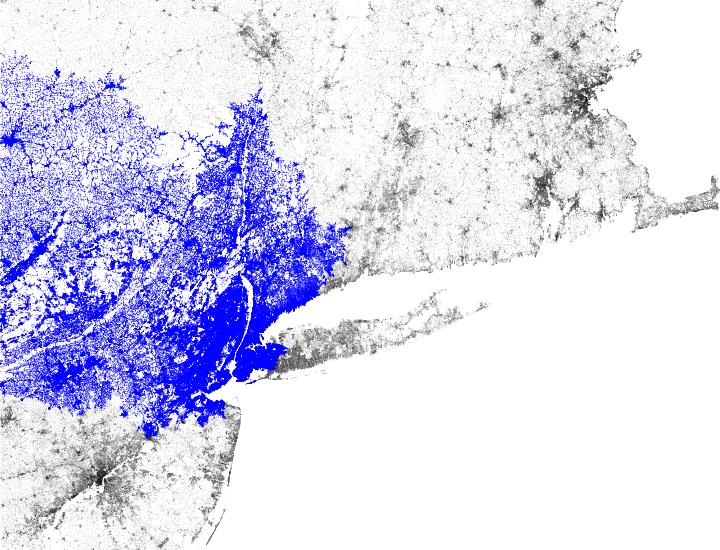
\includegraphics[width=5cm]{figs/incbi-road-ne/singleshot/pgoalnone-balfwd.png}\\556,209 expansions}
%      &
%      \specialcell{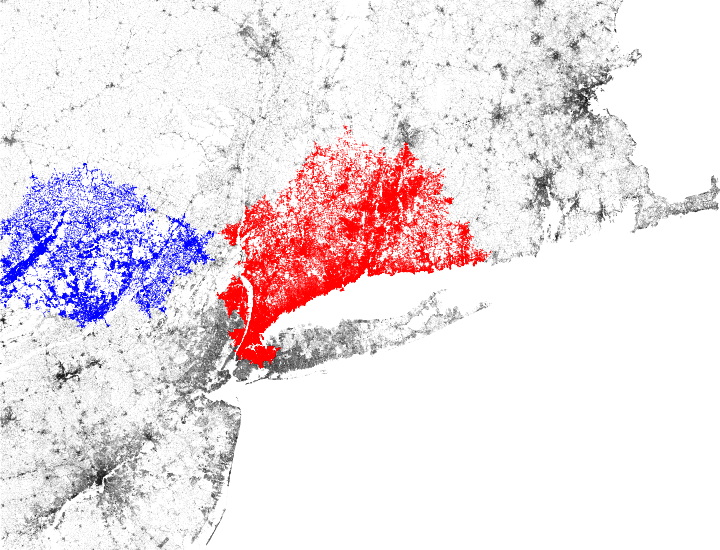
\includegraphics[width=5cm]{figs/incbi-road-ne/singleshot/pavgnone-baldist.png}\\319,938 expansions}
%      &
%      \specialcell{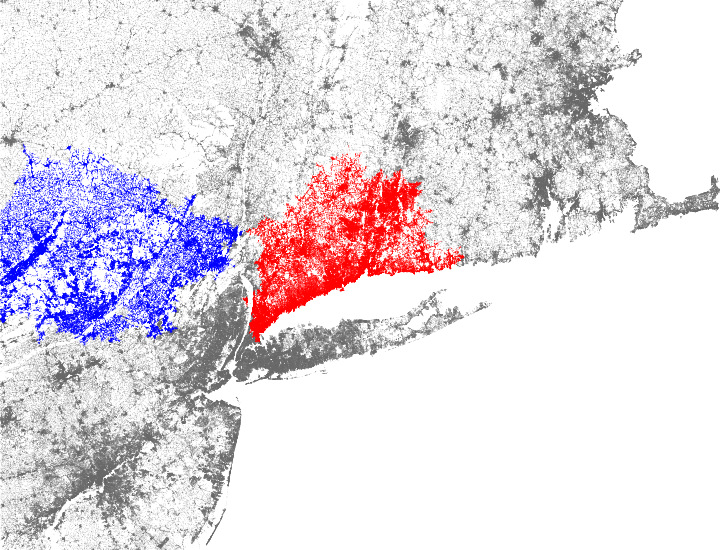
\includegraphics[width=5cm]{figs/incbi-road-ne/singleshot/pavgnone-balcard.png}\\281,413 expansions}
%      \vspace{0.3cm}
%      \\
%      \specialcell{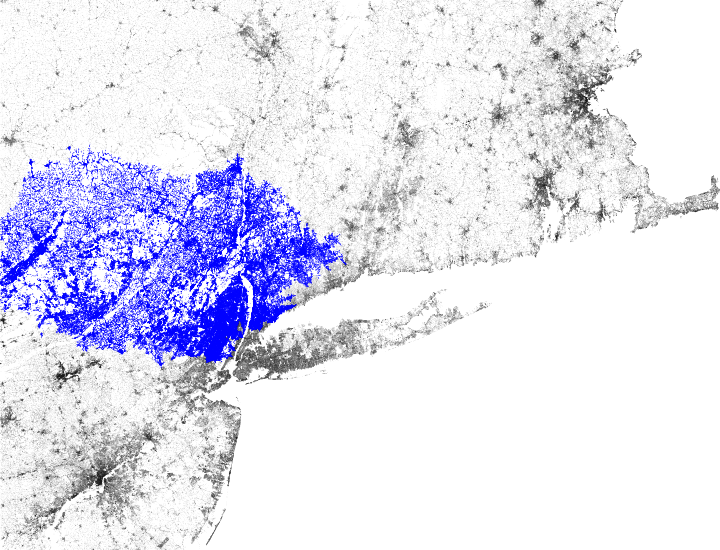
\includegraphics[width=5cm]{figs/incbi-road-ne/singleshot/pgoalhalf-balfwd.png}\\297,414 expansions}
%      &
%      \specialcell{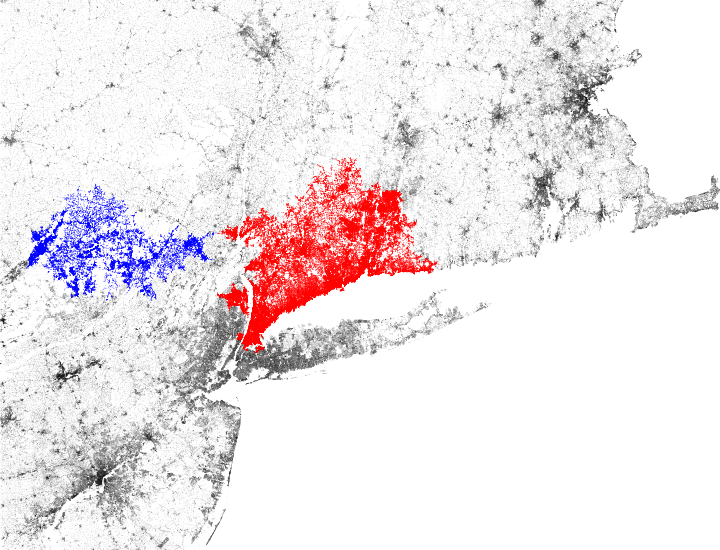
\includegraphics[width=5cm]{figs/incbi-road-ne/singleshot/pavghalf-baldist.png}\\206,625 expansions}
%      &
%      \specialcell{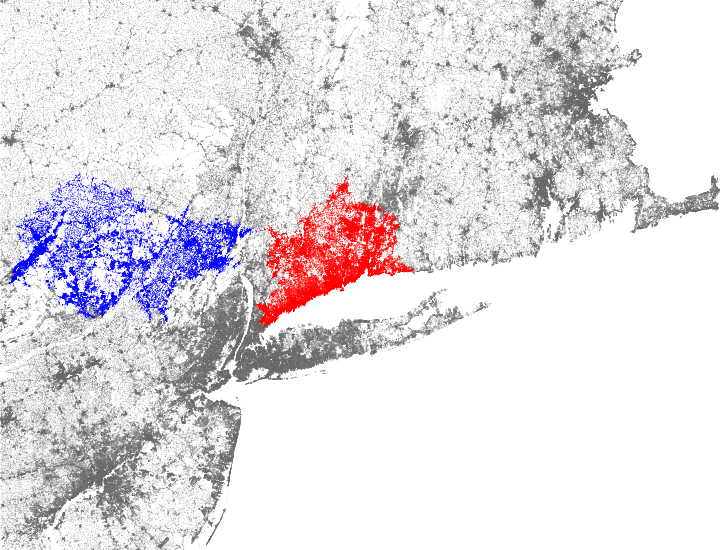
\includegraphics[width=5cm]{figs/incbi-road-ne/singleshot/pavghalf-balcard.png}\\178,929 expansions}
%      \vspace{0.3cm}
%      \\
%      \specialcell{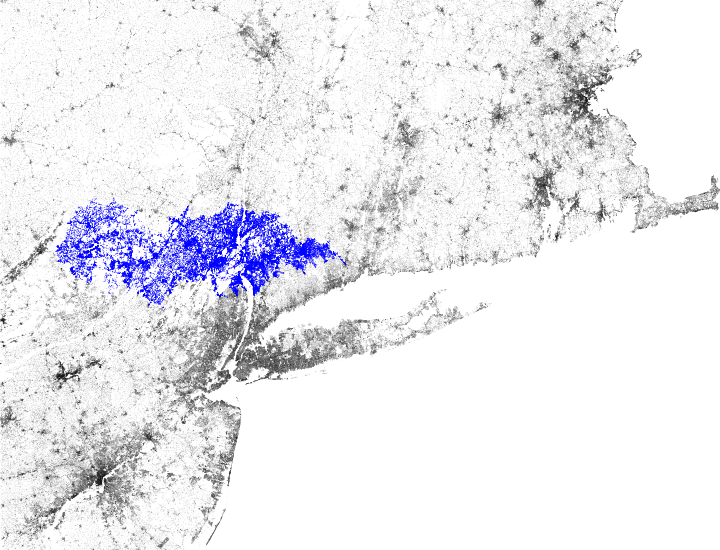
\includegraphics[width=5cm]{figs/incbi-road-ne/singleshot/pgoalfull-balfwd.png}\\82,915 expansions}
%      &
%      \specialcell{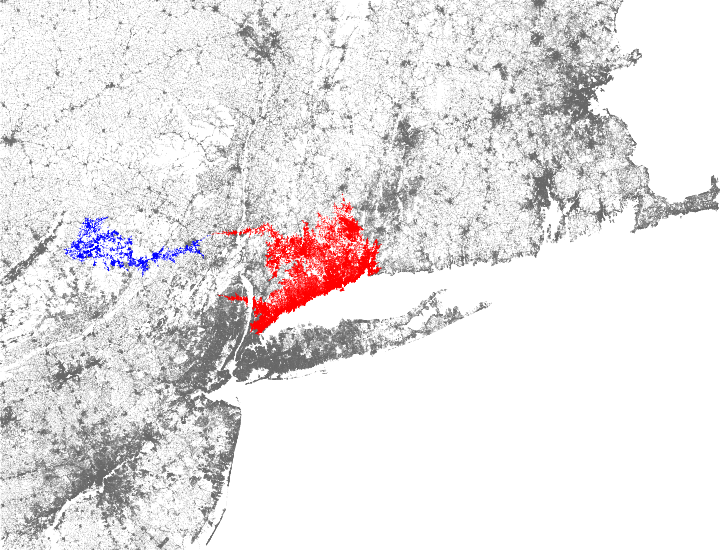
\includegraphics[width=5cm]{figs/incbi-road-ne/singleshot/pavgfull-baldist.png}\\95,759 expansions}
%      &
%      \specialcell{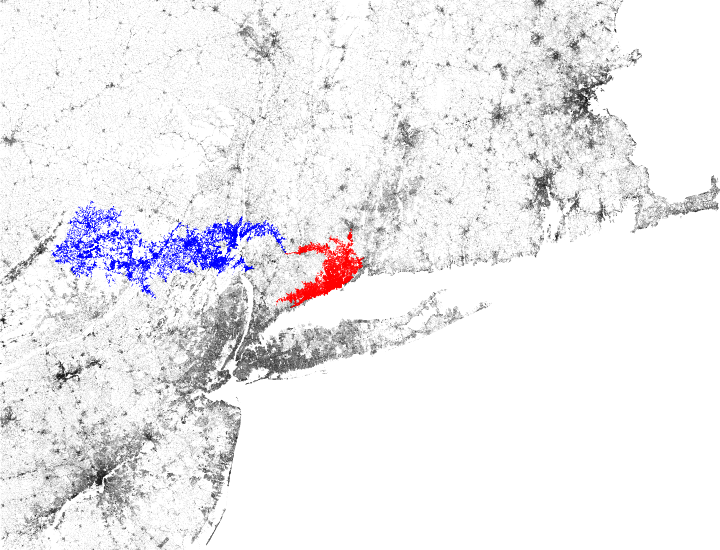
\includegraphics[width=5cm]{figs/incbi-road-ne/singleshot/pavgfull-balcard.png}\\69,218 expansions}
%      \vspace{0.5cm}
%   \end{tabular}
%   
%   \caption{Comparison between various heuristic strengths and
%      balancing strageties on a single-pair road network problem.
%      A path with shortest transit time is sought.
%      The heuristic strength varies from no heuristic (top)
%      to a full-strength heuristic (bottom).
%      At left, a foward-only balancer is used, so that the
%      top-left is equivalent to Dijkstra's algorithm,
%      and the bottom-left is equivalent to A*.
%      The middle column uses a balanced distance strategy.
%      The right column uses a balanced cardinality strategy.}
%   \label{fig:incbi-road-ne}
%\end{figure*}

%\section{Implications for LazySP}

%Gotta talk about this stuff!

%\subsection{LazySP Selector Experiments}

%\begin{figure}
%   \centering
%   \includegraphics{build/incbi-sq/all-even}
%   \caption{Across a selection of articulated robot planning instances,
%      using the Even edge selector.
%      Algorithms are
%      \protect\tikz{\protect\node[fill=black!30,draw=black,postaction={pattern=north west lines}]{};}\;LPA*,
%      \protect\tikz{\protect\node[fill=black!20,draw=black]{};}\;IBiD,
%      and \protect\tikz{\protect\node[fill=black!30,draw=black,postaction={pattern=north east lines}]{};}\;Reverse LPA*.
%      Results shown are cumulative search time.
%      }
%\end{figure}

%\begin{figure}
%   \centering
%   \includegraphics{build/incbi-sq/herbbin0}
%   
%   \includegraphics{build/incbi-sq/herbbin0-lambda}
%   \caption{Problem: \texttt{herbbin0}.
%      Lines are:
%      \protect\tikz{\protect\draw[thick] (0,0) -- (0.15,0.15);} no heuristic,
%      \protect\tikz{\protect\draw[densely dashed] (0,0) -- (0.15,0.15);} start heuristic,
%      \protect\tikz{\protect\draw[densely dashdotted] (0,0) -- (0.15,0.15);} avg heuristic,
%      \protect\tikz{\protect\draw[densely dotted] (0,0) -- (0.15,0.15);} goal heuristic.
%      }
%\end{figure}

%\begin{figure*}
%   \centering
%   \includegraphics{build/incbi-sq/herbbookshelf0}
%   \includegraphics{build/incbi-sq/herbbookshelf1nom}
%   
%   \includegraphics{build/incbi-sq/herbbookshelf0-lambda}
%   \includegraphics{build/incbi-sq/herbbookshelf1nom-lambda}
%   \caption{Problems: \texttt{herbbookshelf0} (left), texttt{herbbookshelf1nom} (right).}
%\end{figure*}

%\begin{figure*}
%   \centering
%   \includegraphics{build/incbi-sq/workcellef}
%   \includegraphics{build/incbi-sq/workcellij}
%   
%   \includegraphics{build/incbi-sq/workcellef-lambda}
%   \includegraphics{build/incbi-sq/workcellij-lambda}
%   \caption{Problems: \texttt{workcellef} (left), \texttt{workcellij} (right).}
%\end{figure*}
